\documentclass[12pt]{article}

%\usepackage{hyperref}
\usepackage[hidelinks]{hyperref}
\usepackage[a4paper]{geometry}					
%\usepackage{ngerman}
\usepackage[utf8]{inputenc}
\usepackage{graphicx}

\usepackage[absolute,overlay]{textpos}
\usepackage{tikz}
\usepackage{url}
\usepackage{eurosym}
\usepackage{amstext}
\usepackage{caption}
\usepackage{subcaption}
\usepackage{listings}
\usepackage{float}

\geometry{hmargin={2.5cm,2.5cm},vmargin={2.5cm,2.5cm}} 	
\geometry{head=1.5cm, foot=1.5cm} 											

\pagestyle{myheadings}
%\markright{Karim Ben Ammar --- }


\begin{document}
%------------------------- Title Page  -----------------------------------
 

\newcommand{\changefont}[3]{\fontfamily{#1} \fontseries{#2} \fontshape{#3} \selectfont}

% coordinates for the bg shape on the titlepage
\newcommand{\diameter}{20}
\newcommand{\xone}{-60}
\newcommand{\xtwo}{440}
\newcommand{\yone}{60}
\newcommand{\ytwo}{-700}


\begin{titlepage}
\setlength{\oddsidemargin}{1cm}
\setlength{\topmargin}{-1cm}


% bg shape
\begin{tikzpicture}[overlay]
\draw[color=gray]
   (\xone pt, \yone pt)
 -- (\xtwo pt, \yone pt)
arc (90:0:\diameter pt)
 -- (\xtwo + \diameter pt , \ytwo pt)
-- (\xone + \diameter pt , \ytwo pt)
arc (270:180:\diameter pt)
-- (\xone pt, \yone pt);
\end{tikzpicture}
\begin{textblock}{10}[0,0](1.5,1.3)
 
\includegraphics[width=.3\textwidth]{KITlogo.pdf}
\end{textblock}
\begin{textblock}{10}[0,0](8.3,1.3)
\begin{flushleft}
\large Institute f\"{u}r Technische Informatik\\
Chair for Embedded Systems
  \end{flushleft}
\end{textblock}

\changefont{phv}{m}{n} % helvetica
\vspace*{3.5cm}
{
\centering
 \huge{Design and Implementation of an IoT-based Control Device for an off-the-shelf Coffee Machine}

 \vspace*{2cm}
 \large{Bachelorarbeit \\
   von
 }\\
 \vspace*{1cm}
 \Large{Karim Ben Ammar}\\
 \vspace*{1cm}
 \normalsize{
 an der Fakult\"{a}t f\"{u}r Informatik\\
 }

\vspace*{3cm}
\normalsize{
\begin{tabular}[ht]{l c l}
   Betreuer: & \medskip  & Prof. Dr. J\"org Henkel\\
  %Betreuender Mitarbeiter: & \medskip & ...\\
   Betreuende Mitarbeiter : &\medskip & Dr.-Ing Lars Bauer \\
   Betreuende Mitarbeiter : &\medskip & M.Sc Farzad Samie \\
   Betreuende Mitarbeiter : &\medskip & M.Sc Marvin Damschen \\
 & & \\
 & & \\
%
%  Die nächsten 2 Punkte werden für Seminare nicht benötigt
%
  Tag der Anmeldung: & \medskip  & 31.1.2017\\
  Tag der Abgabe: & \medskip & 30.05.2017\\

\end{tabular}
}
%\begin{textblock}{10}[0,0](3,14)
%\large{Time: XX.04.2010 \hspace*{0.25cm} -- \hspace*{0.25cm} XX.XX.2009}
%\end{textblock}

}
%\begin{textblock}{10}[0,0](1.75,15.365)
%\tiny{
% KIT -- Universit\"{a}t des Landes Baden-W\"{u}rttemberg und nationales Forschungszentrum in der Helmholtz-Gemeinschaft
%}
%\end{textblock}

\begin{textblock}{10}[0,0](9.7,14.95)
Chair for Embedded Systems
 
\includegraphics[width=.07\textwidth]{CESlogo.pdf}
\end{textblock}


\end{titlepage} 

  \thispagestyle{empty}
  \pagebreak
  \afterpage{\null\newpage}
\topskip0pt
\vspace*{\fill}
\textbf{\LARGE{Selbstst\"andigkeitserkl\"arung}}
\bigbreak
\bigbreak
\bigbreak
\bigbreak
Ich versichere, dass ich die vorliegende Arbeit selbstständig angefertigt und
mich keiner fremden Hilfe bedient habe. Alle Stellen, die wörtlich oder
sinngemäß veröffentlichtem oder unveröffentlichtem Schrifttum entnommen
sind, habe ich als solche kenntlich gemacht.
\bigbreak
\bigbreak
\bigbreak
\bigbreak
\noindent\rule{\textwidth}{0.4pt}
Karlsruhe 30.05.2017
\vspace*{\fill}
\clearpage
\begingroup
  \pagestyle{empty}
  \null
  \newpage
\endgroup
\topskip0pt
\vspace*{\fill}
\begin{abstract}
    We live in a world evolving at an incredible pace. 
    New technologies to facilitate our daily life are being developed : Smart homes where a person can interact with his house, fridge lights etc.
    Having an interactive environment around us is not a luxury anymore, but a commodity to improve our daily tasks. 
    The main idea behind this project is to give a second life to our not so “interactive”  instruments. 
    We want to control them and monitor them in a modern way. 
    For this purpose an RFID based authentication system will be developed in order to prevent unauthorized users from using the machine. 
    Another feature, would be to automatically detect the user's order and charge him accordingly.
    A Logging/Debugging system should be implemented in order to help the admin user,
    detect and have a better understanding of any strange behaviour that may occur on the coffee machine.
 \end{abstract}
\vspace*{\fill}
\pagebreak
\topskip0pt
\vspace*{\fill}
\begin{abstract}
 In einer Welt wo die Technologien sich schnell entwickeln, bietet sich immer die Möglichkeit diese neuen Technologien zu verwenden um den Alltag von den Menschen einfacher zu machen.
 Diese Bachelorarbeit hat als Ziel eine Kaffeemaschine mit einem intelligenten System zu verbinden um den ganzen Process von Kaffeebestellungen zu modernisieren.
 Hierzu wird erstens ein Authentifizierungssytem basierend auf RFID Tokens gebaut, um unerlaubte Benutzerzugriffe zu vermeiden. 
 Zweitens, wird eine internet-basierte Zahlungsmethode mit der automatischen Erkennung von den Bestellungen kombiniert.
 Letztens, wird ein Monitoring-System entwickelt, das das Verhalten der Kaffeemaschine in ihren verschiedenen Zuständen protokolliert.
 \end{abstract}
\vspace*{\fill}
\pagebreak
%-------------------------- Inhaltsverzeichnis ----------------------------
	\tableofcontents
  \thispagestyle{empty}
  \pagebreak
  
 \listoffigures 
 \clearpage
\begingroup
  \pagestyle{empty}
  \null
  \newpage
\endgroup
\noindent
\textbf{ \LARGE{Acronyms}} \\~\\
\textbf{RFID} Radio-Frequency Identification\\~\\
\textbf{NFC} Near Field Communication\\~\\
\textbf{UID} Unique Identifier \\~\\
\textbf{SPI} Serial Periphal Interface\\~\\
\textbf{FSM} Finite-state machine\\~\\
\textbf{GPIO} General-purpose input/output\\~\\
 \clearpage
\begingroup
  \pagestyle{empty}
  \null
  \newpage
\endgroup
%------------------------------ Hauptteil ---------------------------------

  \setcounter{page}{1}


  \section{Introduction}

    
    In a workplace, a common meeting spot for coworkers is around the coffee machine.\\
    The main problem when having an off-the-shelf machine, is the administrion of the user's behaviour. 
    Using tally sheets can be troublesome and error-prone : Endless counting, the user forgets to write down his/her transaction, etc.
    An automated solution is needed in order to identify each user, and charge him/her according to his/her order, avoiding any third-party's involvement in the process. \\
    
    This work is an improved and extended replacement for an older project, which upgraded an automatic coffee machine.
    The main idea was to add an interactive user control, and facilitate the payment method. 
    Our goal is to clarify some dark corners left by the previous work which was too complex.
    Therefore, the goals of this work are to provide a simple setup with a user-friendly interface to perform the user-specific accounting using RFID tags, 
    when ordering a coffee. Furthermore, debugging mechanism (logging, remote diagnostics) should be put in place,
    e.g., to be able to observe unexpected inputs from the coffeemachine (to the accounting system) 
    
  \subsection{Requirements}
  The final product should present the following features : \\
  \begin{itemize}
  \item The system should keep the coffee locked, and only unlocks it for registered users

  \item The authentication system is based on RFID tokens, which are available in many forms (e.g. KIT student/employee cards, gym cards, etc)
 
  \item Each user has to be registered in the preexisting accounting server, in order to use the system, where every user can attach any number of RFID tokens to his account

  \item The user should be able to order coffee with the main application (Raspberry Pi) or his android Smartphone, using a user friendly and intuitive interface

  \item After unlocking the coffee machine, the system should detect the user's order and charge him accordingly
  
  \item If the internet connection is not available, the transactions should be stored locally. 
  The offline transactions should be transmitted to the server, when the internet connection is back.
  
  \item The system should be able to monitor signals of the coffee machine and save them. This data will be used to define the different states of our machine and detect any unusual behaviour.
  \item The system should be easy to use and upgrade
  \item The system should log the behaviour of the coffee machine, providing the administrator all needed information in order to debug any strange behaviour.
   \end{itemize}
   \pagebreak
   \subsection{Structure of this work}
   
   In chapter 2, the preexisting hardware and software used in this project are discussed.
   Chapter 3 presents the main features of this work, the upgraded hardware, the new software, how they were designed and implemented.
   Chapter 4 summarizes this work, and gives an outlook.


  \section{Foundations}
  In this chapter we will introduce the foundations of the project.
  \subsection{Coffee machine}
  \subsubsection{Overview}
  For this work, we will use a Saeco Royal Cappuccino (SUP016R) coffee machine (see figure \ref{fig:coffeeMachine}) as our main device. 
  This is a fully automatic coffee machine which allows the brewing of either cappuccino or normal coffee. 
  This machine also offers hot water and steam if needed.\\~\\
  \begin{figure}[h]
   \centering
   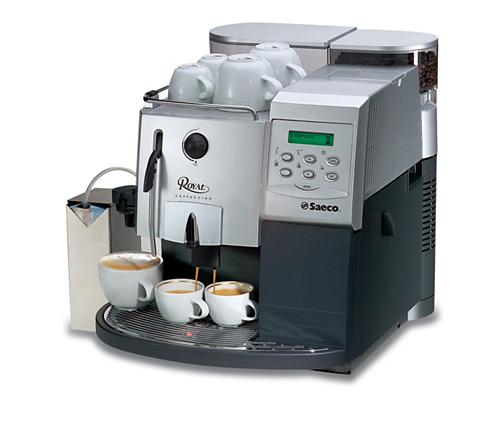
\includegraphics[width=8cm, height=7cm]{./images/coffeeMachine}
   \captionsetup{justification=centering}
   \caption{Saeco Royal Cappuccino (Taken from \cite{SaecoPic})}
   \label{fig:coffeeMachine}
  \end{figure}
  In order to fulfill the requirements described above, the coffee machine needs to be locked until an authorized user logs in.
  A better understanding of the machine (grinding, brewing cycles etc) is required if we want to create a good monitoring system.
  Due to the variety of beaverages offered by the coffee machine, and different processes that the user can manipulate, 
  the machine's sensors are used as a way to differentiate between the multiple scenarios.
  The different sensors are located on the right side of the coffee machine. They can be easily accessed after removing the case.
  A better upgrade would be to control the coffee machine directly, unfortunately the button board is secured on the inaccesible side of the board, and
  therefore we used the different sensors as an ordering mechanism in this work. The Saeco International Group has a service manual\cite{Saeco} for the different Royal products.
  This document describes the behaviour of the coffee machine providing details about every sensor.
  \newpage
  \subsubsection{Workflow}
  In order to provide an optimal user experience, we need to have a better understanding of the coffee machine. 
  We can devide the coffee ordering mechanism in two main processes : Preparation phase and the order phase.\\~\\
  \textbf{Preparation phase:}\\
  
  The coffee machine uses internally a gear motor, which turns a large gear wheel in order to move between the different states (For further details please refer to \cite{Saeco}).
  First the gear motor is initialised and moves to home position followed by the activation of the water heater for one and a half minute. 
  This would heat the water to the desired temperature coninuously for 60sec and then is alternated for the remaining period fo time.\\~\\
  \textbf{Ordering phase:}\\
  
  After pressing the start button, the grinder is triggered for 5.5 sec, followed by two consecutive activations of the doser. 
  The gears change to brewing position, and the pre-brewing begins followed by the brewing process. The duration depends on the coffee selected. 
  Finally, the gears move back to home position. A summary of the whole process can be viewed in figure \ref{fig:timingCoffee}
  \begin{figure}[h]
   \centering
   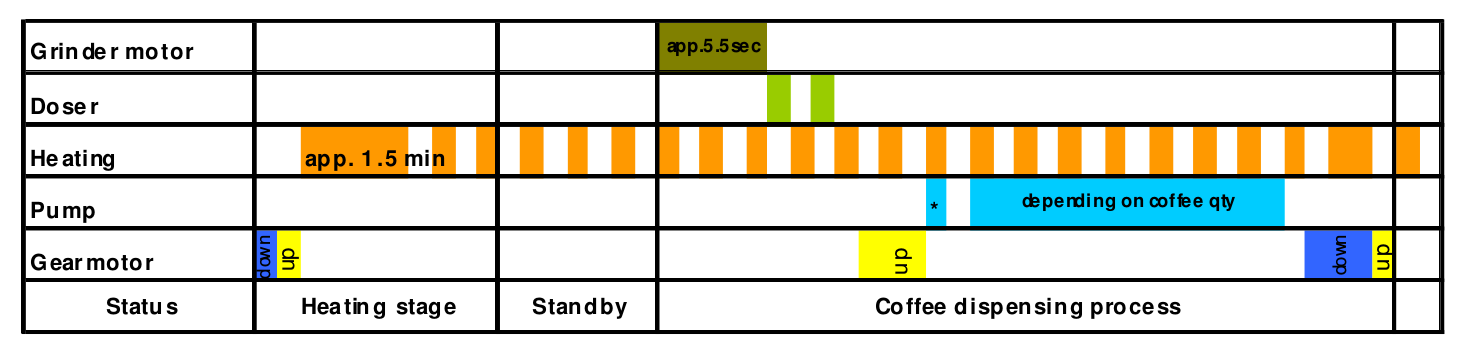
\includegraphics[width=16cm]{./images/timing}
   \captionsetup{justification=centering}
   \caption{Coffee ordering process (taken from \cite{Saeco}) }
   \label{fig:timingCoffee}
  \end{figure}
  
  \subsubsection{Electrical connections}
  As depicted in figure \ref{fig:machinePins}, the coffee machine has multiple sensors. For this project, we will use the input of the last four sensors :
  \begin{itemize}
  \item Flow meter system 1 : For water usage detection
  \item Flow meter system 2 : For water usage detection
  \item Reed switch water level : For low water level detection
  \item Doser switch : For coffee detection
  \end{itemize}
  
  \newpage
  \textbf{Flow meter sensors :}\\
  
  The flow sensors have each three pins, used as follows :
  
  \begin{table}[ht]
  \begin{minipage}[b]{0.56\linewidth}
    \centering
  \begin{tabular}{lllr}
   \hline
  Wire & & &Type \\
  \hline
  Green wire & & &5V \\
  Brown wire & & &Ground\\
  Yellow wire & & &Output\\
  \hline
  \end{tabular}
  \end{minipage}\hfill
  \begin{minipage}{0.4\linewidth}
  \centering
  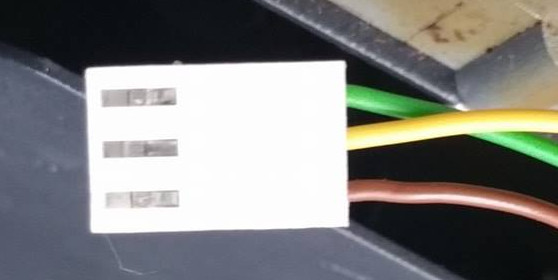
\includegraphics[width=40mm]{./images/realPins}
  \captionof{figure}{Flow sensor}
  \label{fig:realPins}
  \end{minipage}
  \end{table}
  
  These sensors monitor the flow rate: They control the water quantity delivered for the different beverages. 
  When an order is detected, the system will inspect the flow meter if it is turning.
  According to \cite{Saeco} , if no signal is detected within 10 seconds, the cycle is stopped, and a warning message is displayed.\\
  \begin{figure}[H]
   \centering
   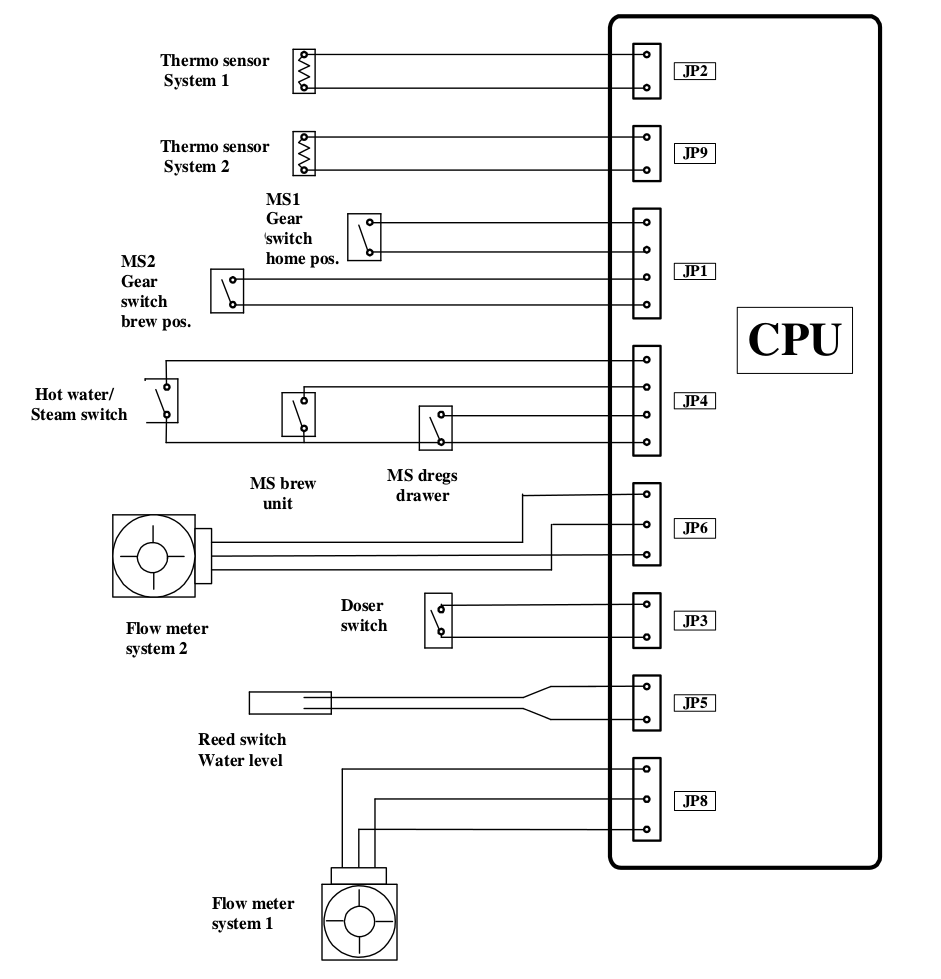
\includegraphics[height=16cm]{./images/machinePins}
   \captionsetup{justification=centering}
   \caption{Coffee machine electrical board (taken from \cite{Saeco})}
   \label{fig:machinePins}
  \end{figure}
  \textbf{Water level/Doser switches :}\\
  
  As pictured in figure \ref{fig:waterDoser}, both switches will pull the pin to ground when activated.
  For water level detection, a reed switch is used. The switch's mechanism is made from two seperate components. The first one is the magnet. 
  It is floating inside a small chamber in the water tank. This provides him the necessary freedom to follow the water level. 
  The second part is the actual switch placed at the same level with the magnet. 
  Whenever the water drops under a certain threshold, the switch would be no longer controlled by the magnet, and trigger the low water level signal. 
  This will lock the coffee machine temporarly, until the water tank is refilled. 
  This signal will be simulated in our work by the Raspberry Pi, in order to keep the coffee machine locked.
  
 
  
   \begin{figure}[H]
   \centering
   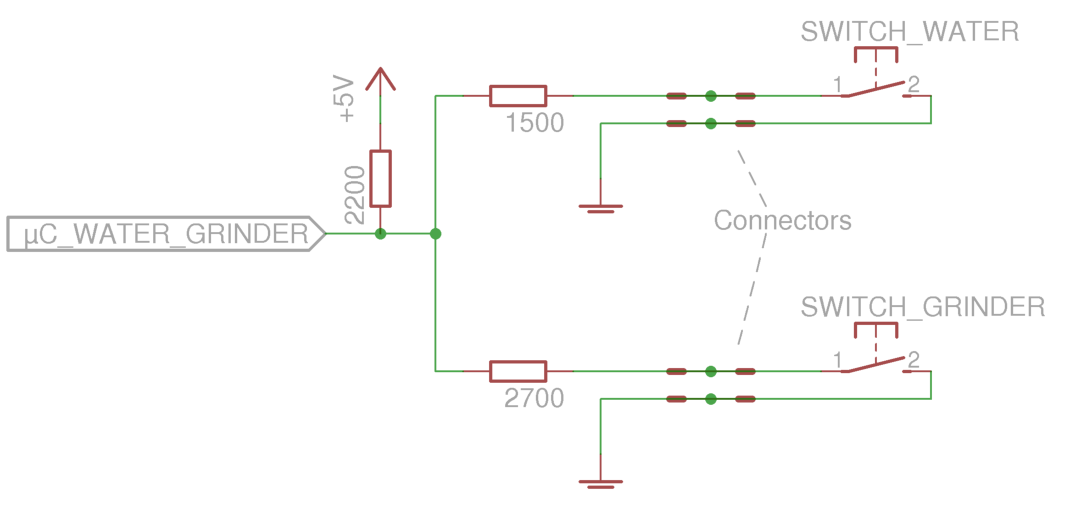
\includegraphics[width=14cm]{./images/waterDoser}
   \captionsetup{justification=centering}
   \caption{Electrical representation of the water and doser switches (taken from \cite{BachelorThesis})}
   \label{fig:waterDoser}
  \end{figure}
  
  \subsection{Accounting system}
  The order transactions are managed by a preexisting accounting system. 
  The user has to register and add money to his account in order to use the provided system. 
  After ordering his beverage, the user has to inform the system about his transaction. 
  Different methods were implemented for this purpose. The currently used procedure consists of printed tally sheets.
  The user has to write down his transaction by adding a mark in front of his name. 
  The sheets are checked periodically, and the corresponding accounts are updated accordingly. 
  The second method consists of a web interface. In this project, we will use this approach.
  Every user is identified by a unique ID, which will be used in every transaction. 
  This method gives the administrator more control over the transactions (Less counting mistakes, and set a limit for negative balances).
  Plus, the user has the possibility to consult his consumption statistics and history after each order.

  \pagebreak
  
  \section{Design/Implementation}
  
  \subsection{User Interaction}
  The developed system has to ensure the workflow pictured in figure \ref{fig:workflow}.
  Any user has the possibility to consult the entertainment content (comic pictures) without the need to identify himself. This will be viewed more in details in section \ref{sec:raspberry}.
  The coffee machine has to remain locked, preventing any order, until the user presents his RFID token.\\
  If the user is registered, and his balance is above a certain threshold, the coffee machine will be unlocked, otherwise the user will be asked to register his RFID token before retrying.
  This can be done by the coffee administrator. When an invalid token is detected, a custom window with the user's UID should popup. This will facilitate the registration task for the admin.\\
  Once the coffee machine is unlocked, the user can either press the coffee button or the water button. A distinct button has to be provided to the user regarding his milk preferences.
  The system should automatically detect the chosen beverage and charge the user accordingly. The accounting page should be visible only to valid users.
  The machine has to return to the locked state as soon as the user receives his order.
  
   \begin{figure}[H]
   \centering
   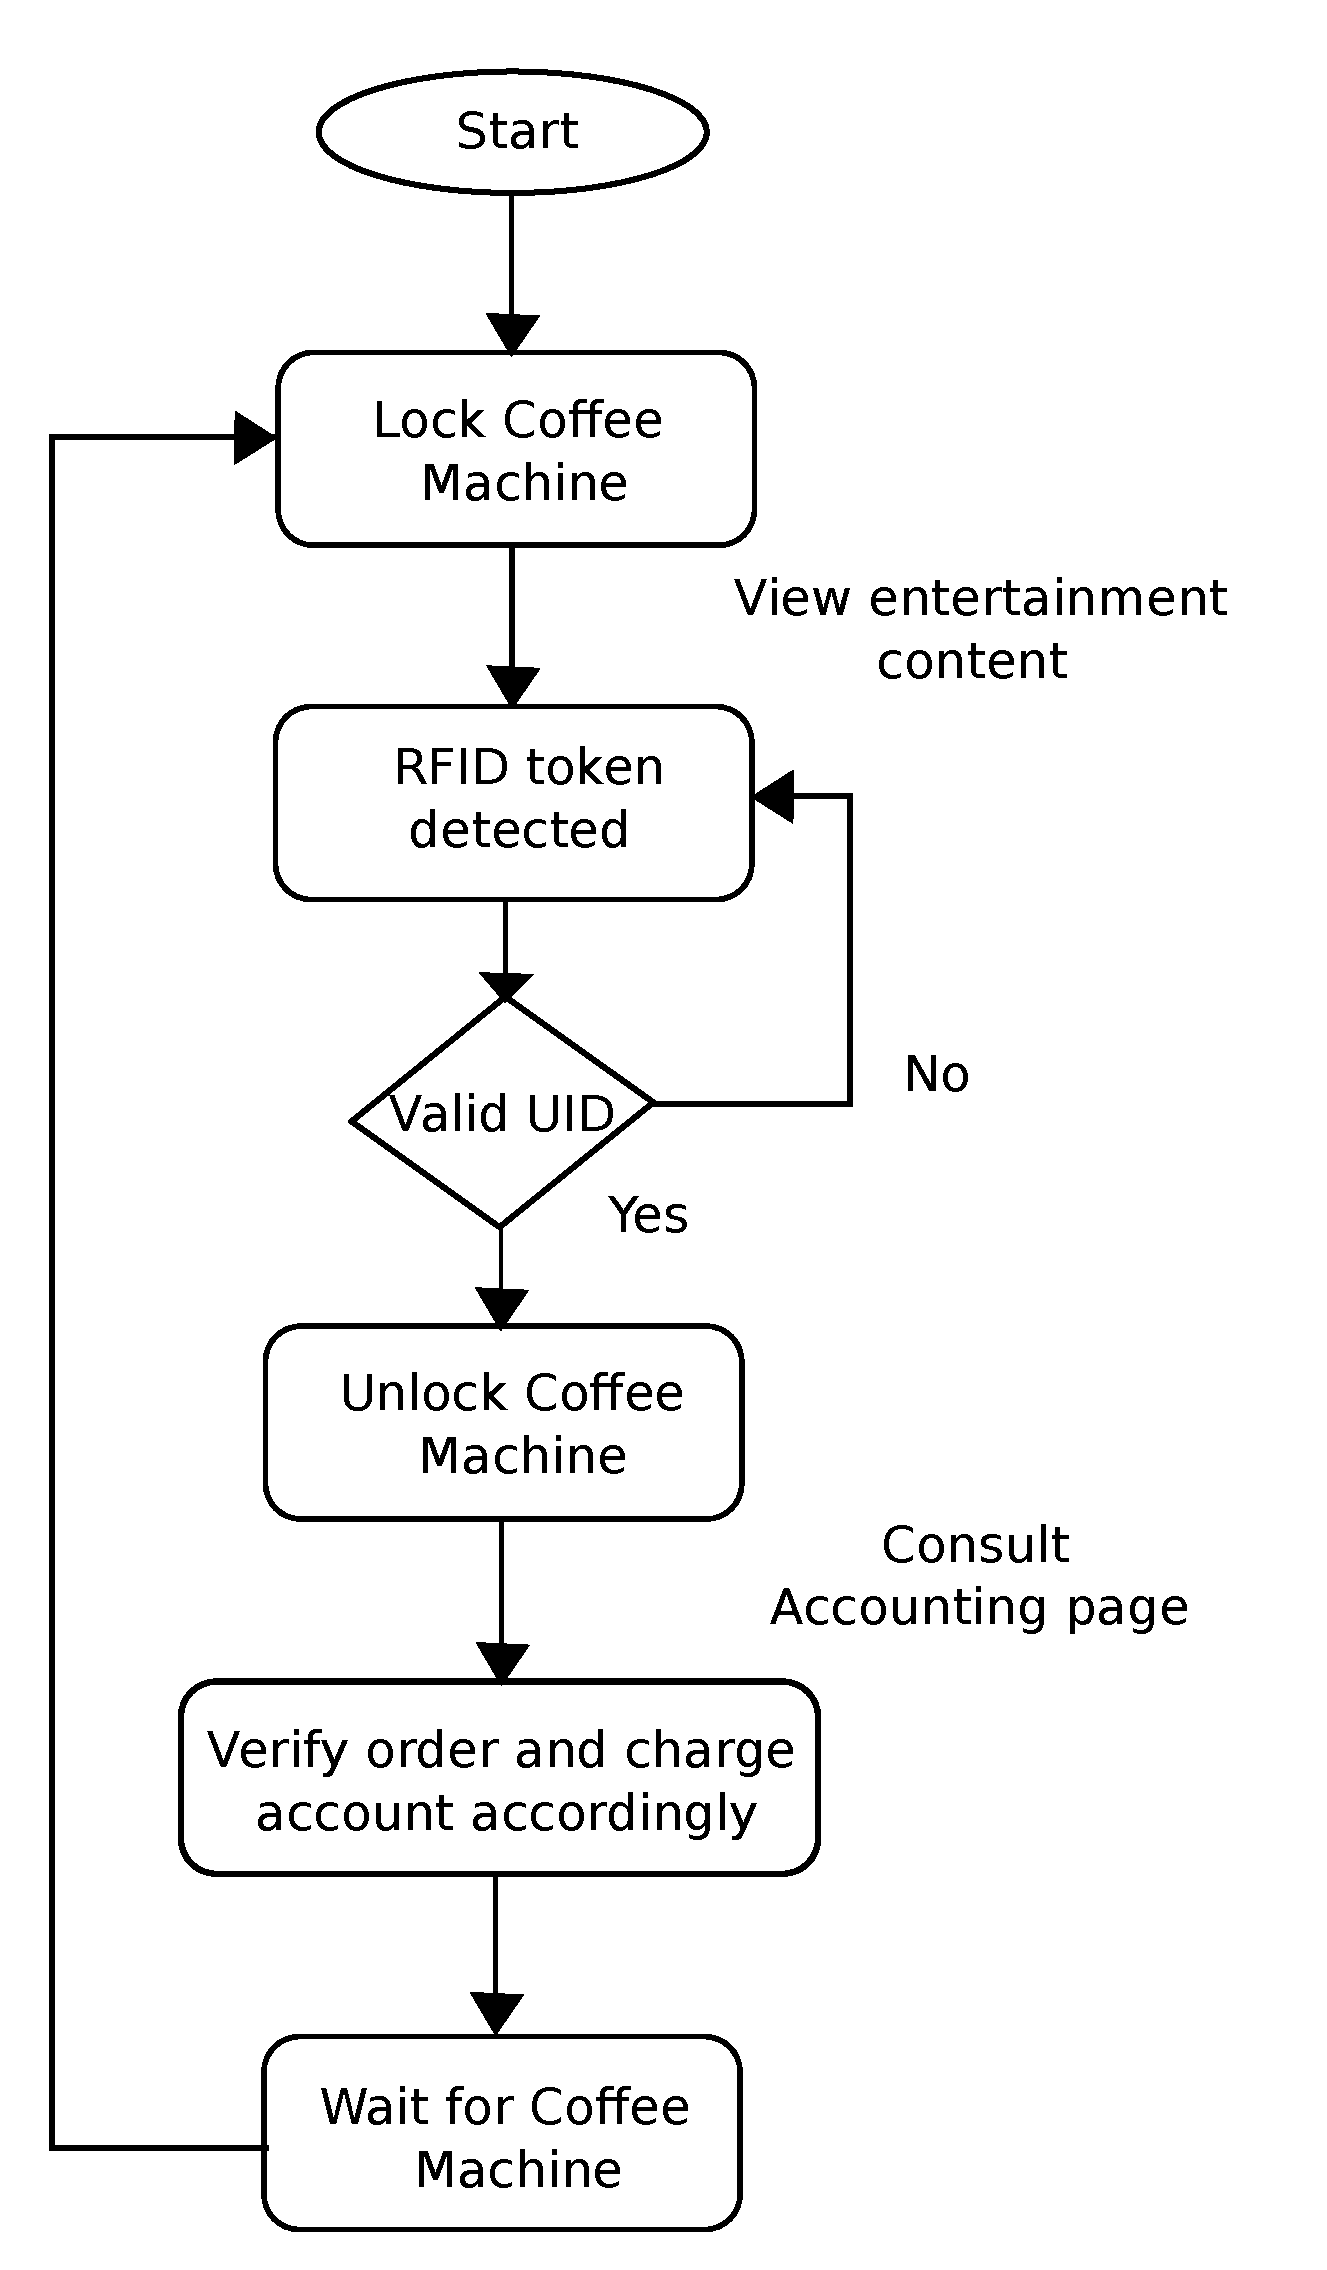
\includegraphics[height=14cm]{./images/workflow}
   \captionsetup{justification=centering}
   \caption{User interaction workflow}
   \label{fig:workflow}
  \end{figure}
  \subsection{Hardware}
  In order to provide the best user experience with this project, we have to take into consideration some criteria when choosing the hardware.
  Over the past years, a new trend of mini-computers appeared : NanoPi 2 Fire, Raspberry pi, NanoPC-T3 etc \\
  For our system, we will use a Raspberry Pi, the official pi 7\,'' touchcscreen (see figure \ref{fig:touchscreen}) and the Joy-IT RFID Modul.
   \begin{figure}[H]
   \centering
   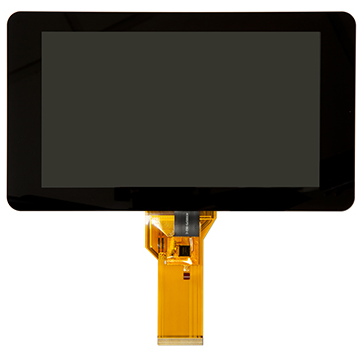
\includegraphics[width=6cm, height=6cm]{./images/touchscreen}
   \captionsetup{justification=centering}
   \caption{Official Raspberry Pi 7\,'' touchscreen \cite{touchScreen}}
   \label{fig:touchscreen}
  \end{figure}
  
  \subsubsection{Raspberry pi}
   In this project, we will use a Raspberry Pi 3 model B (see figure \ref{fig:raspberry}) as our main controller for several reasons :
   \begin{itemize}
  \item Affordable
  \item Provides a GPIO interface
  \item Characteristics : Despite the small size, the Raspberry Pi is considered as a mini-computer
  \item Linux based operating system (RASPBIAN)
  \item No need for extra hardware for internet connectivity
  \end{itemize}
  
   \begin{figure}[H]
   \centering
   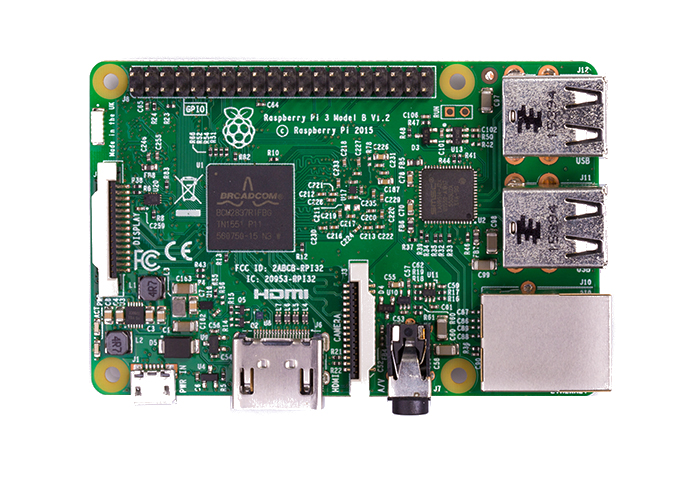
\includegraphics[width=6cm]{./images/raspberry}
   \captionsetup{justification=centering}
   \caption{Raspberry pi 3 model B (taken from \cite{raspberryPi3})}
   \label{fig:raspberry}
  \end{figure}
  
  The currently used Raspberry Pi features a 1.2GHz 64-bit quad-core ARMv8 CPU, 1GB RAM, 4 USB ports, and 40 GPIO pins.
  It also provides a Bluetooth 4.1 interface that can be used for future upgrades to the system.
  For a better user experience and due to the lack of display, we attached a 7\,'' LCD touchscreen to the Raspberry Pie.\\
  A custom PCB was made to permit the communication between the Raspberry Pi and the coffee machine. 
  This will prevent eventual damages due to the difference between voltages.\\
  With this solution, we should be able to receive/send data from/to the coffee machine.\\~\\
   \subsubsection{RFID Reader}
  For authentication purpose, we will use RFID tokens. They can be extracted from any RFID emitter ex. KIT employee/student card.
  In order to read the token's UID, we will use a Joy-IT RFID Module (see figure \ref{fig:RFID}). This works perfectly with the Raspberry Pi.
  The RFID reader is directy connected to the GPIO Board on the Raspberry Pi using the SPI as a communication interface. 
  
  \begin{figure}[H]
   \centering
   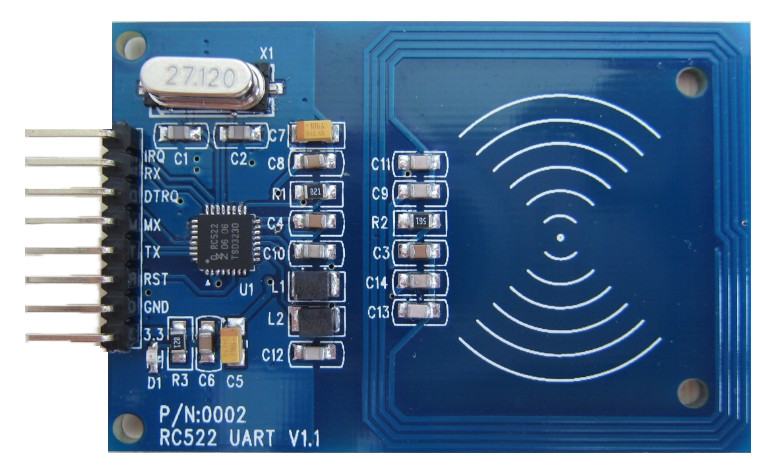
\includegraphics[width=6cm, height=4cm]{./images/rfid}
   \captionsetup{justification=centering}
   \caption{Joy-IT RFID-RC522 Module (taken from \cite{rfidJoy})}
   \label{fig:RFID}
  \end{figure}
  \textbf{GPIO pins:}\\
  
  As shown in figure \ref{fig:raspberryGPIO} the Raspberry Pi has 40 different GPIO pins. For this project, we will need 22 of them to manage the different parts of our build.
  The RFID reader must be connected to specific pins which use the SPIO interface. 
  As shown in Table \ref{tab:rfidGPIO}, each pin from the RFID reader has to be connected to a certain pin on the Raspberry Pi.
  \begin{table}[H]
  \centering
  \begin{tabular}{llr}
   \hline
  Raspberry Pi pin & RFID reader pin\\
  \hline
  GPIO 8 & SDA\\
  GPIO 9 & MISO\\
  GPIO 10 &  MOSI\\
  GPIO 11 & SCK\\
  GPIO 25 & RST\\
  Ground & GND\\
  3V3 & 3.3V\\
  \hline
  \end{tabular}
  \caption{Pin connections between the RFID reader and the Raspberry Pi}
  \label{tab:rfidGPIO}
  \end{table}
  For the screen, one 5V pin and one Ground pin are needed. In this upgrade, a Buzzer was added to notify the user. This needs one Ground pin and one free output pin.
  For the sensors output, 11 pins are required. Two of them are reserved to a 3V3 pin and a Ground pin. The pin's configuration will be explained further in section \ref{pcb}
  
   \begin{figure}[H]
   \centering
   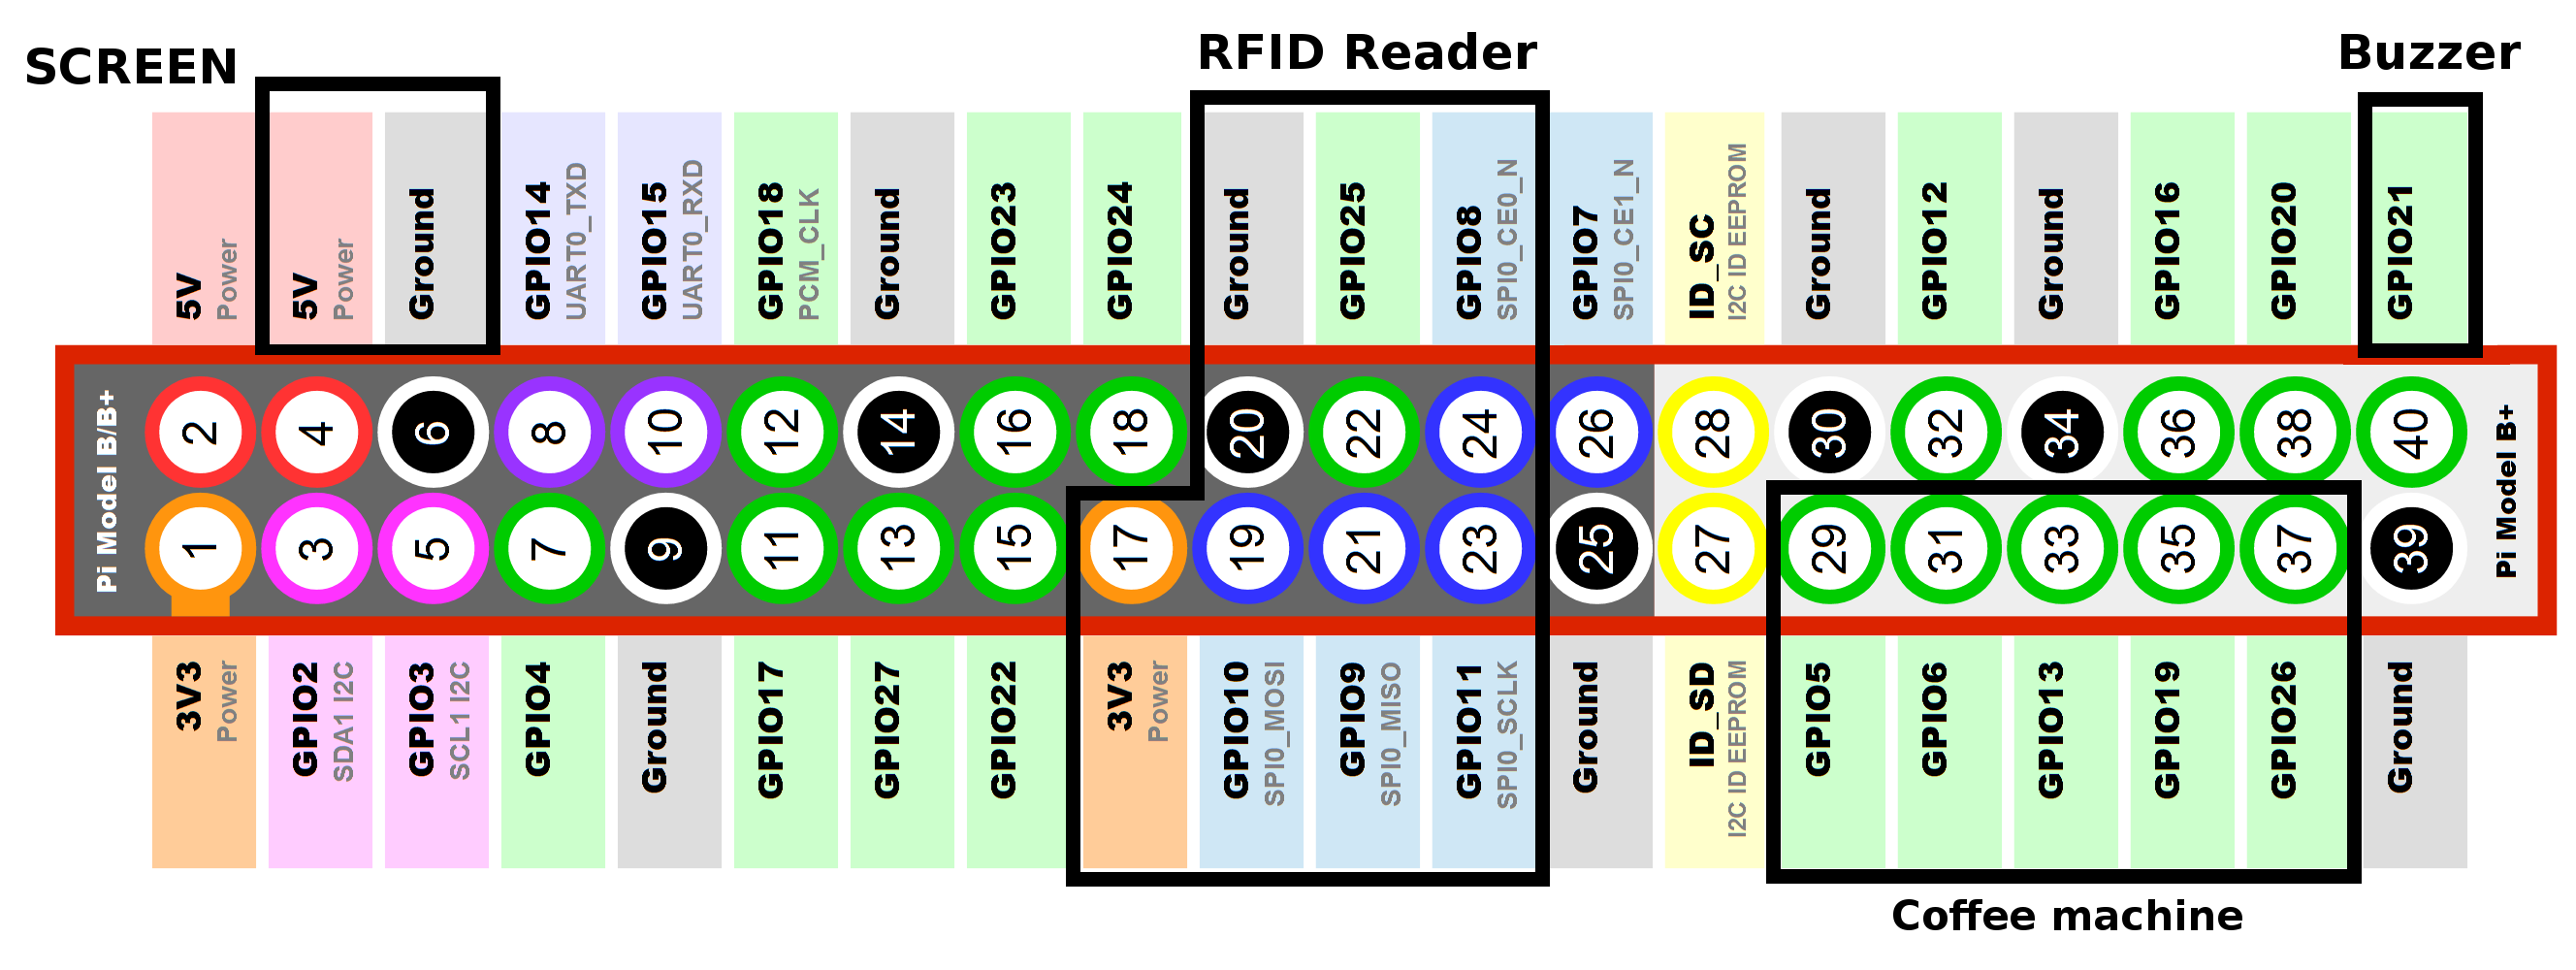
\includegraphics[width=1.0\textwidth]{./images/raspberryGPIO}
   \captionsetup{justification=centering}
   \caption{Raspberry Pi GPIO Board (taken from \cite{gpioBoard})}
   \label{fig:raspberryGPIO}
  \end{figure}
  
  
  \subsubsection{Adapter Coffee Machine/Raspberry Pi} \label{pcb}
   \begin{figure}[H]
   \centering
   \includegraphics[width=8cm]{./images/oldPCB.pdf}
   \captionsetup{justification=centering}
   \caption{Adapter Coffee Machine's side (taken from \cite{BachelorThesis})}
   \label{fig:realpcb}
  \end{figure}
  Due to the difference in voltage between the Raspberry Pi and the coffee machine, a custom PCB has been created.
  One version of the PCB which can read the input of upto 9 sensors has been developed. Unfortunately, this version had a strange behaviour.
  The corresponding schematic can be viewed in the appendix section. The currently used PCB reads the output of 4 different sensors.
  It uses optocouplers to transfer the coffee machine's output to the Raspberry Pi and the locking signal in the other direction. 
  This isolates the two systems preventing any accidental damage to the components.
  The adapter is made from two seperate parts connected by 5 pins cable.
  The board on the coffee machine's side uses one four-channel Avago ACPL-247 optocoupler for the different sensors output and one single-channel Avago ACPL-217 
  for the lock/unlock signal.\\
  %As shown in figure \ref{fig:pcb} the Raspberry-facing part will be directy plugged on top of the Raspberry Pi. This prevents unexpected connection problems.
  %The pins on the upper side are reserved. They will be used for the different external components :\\
  %\begin{itemize}
  % \item The two pins labeled 5V and GND will be connected with the screen. 
  % \item The 7 pins in the middle are reserved for the RFID Reader
  % \item The last two pins are used to control the Buzzer
  %\end{itemize}
  %The pins on the bottom side of the pcb will be directly connected to the adapter on the coffee machine's side with a 14 pins cable.
  %For the different inputS coming from the coffee machine, we need 9 pins. Two additional pins ( GND and 3V3 ) are used by the optocouplers.
  
  %\begin{figure}[H]
   %\centering
   %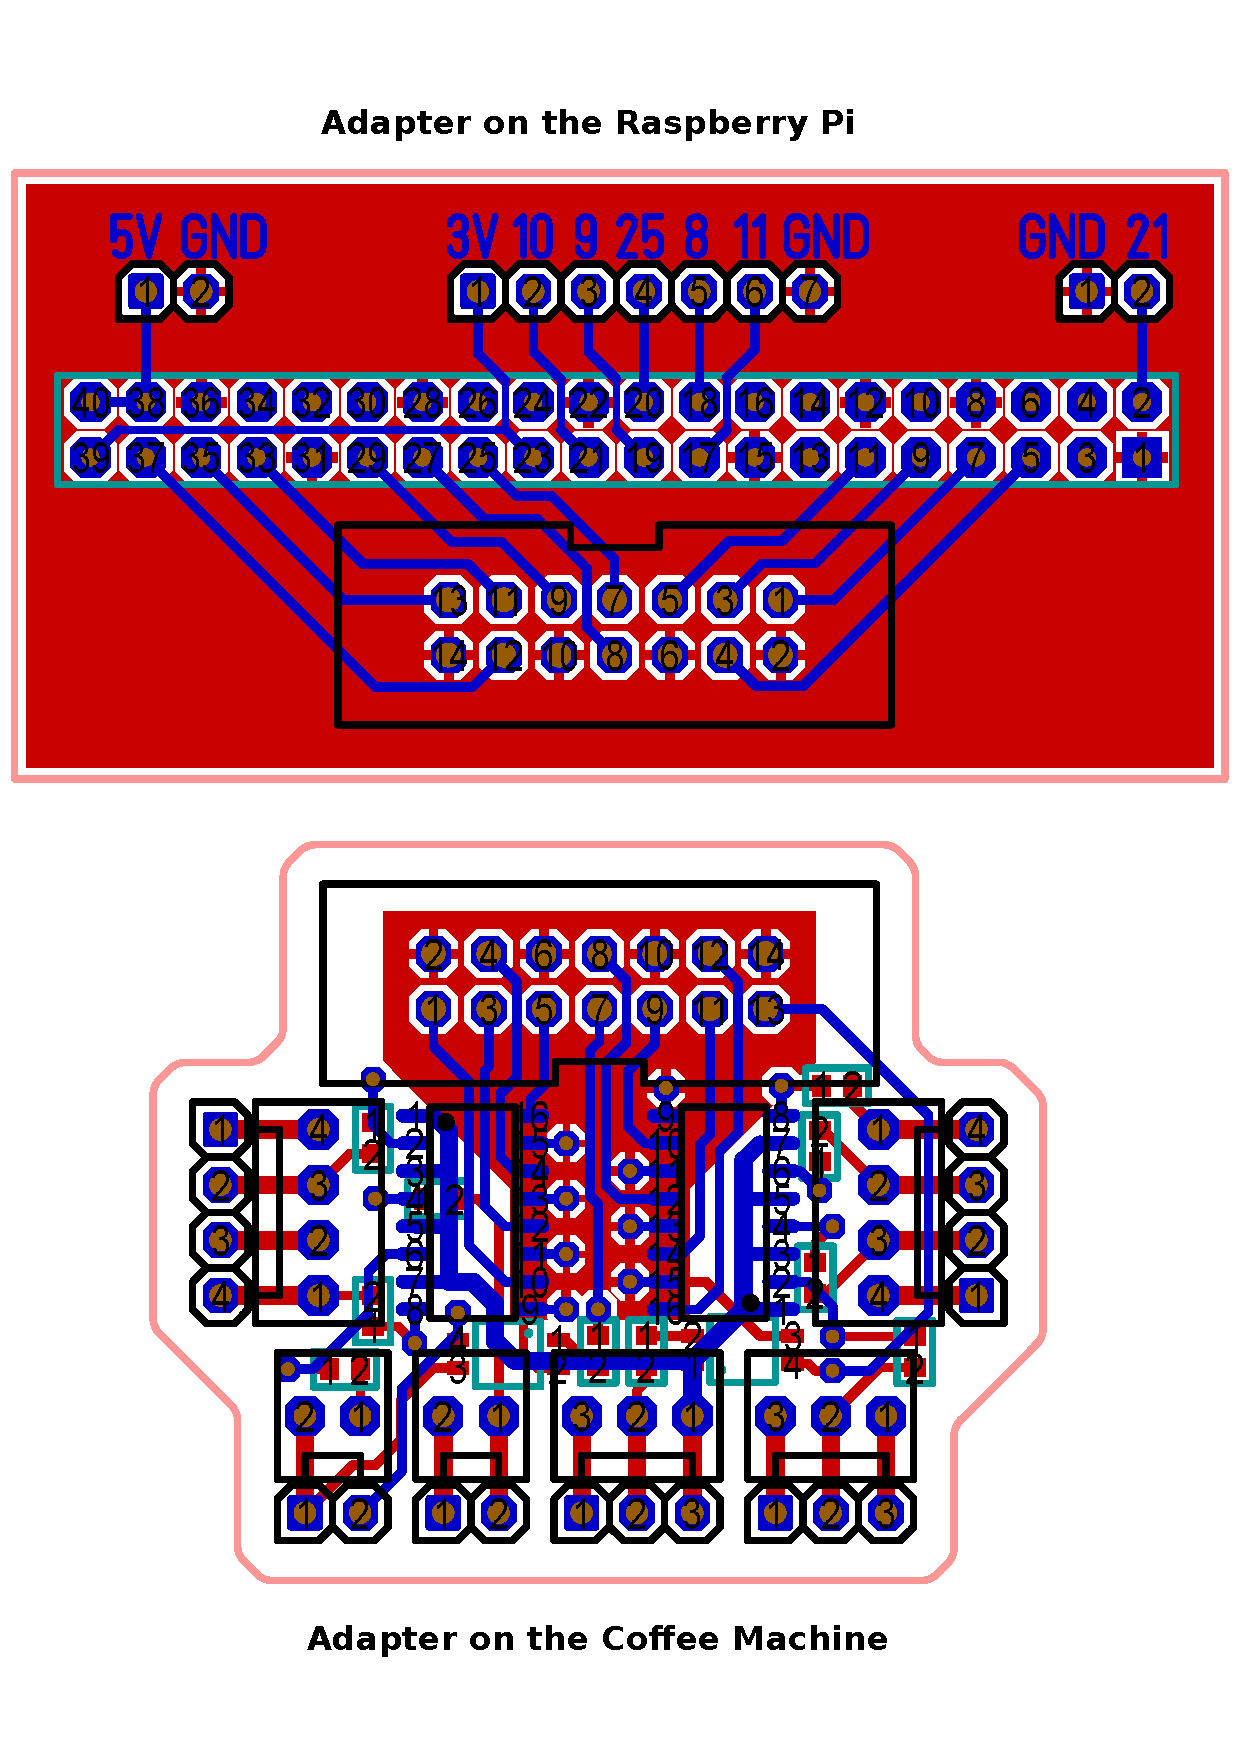
\includegraphics[width=14cm]{./images/pcb}
   %\captionsetup{justification=centering}
   %\caption{Adapter Coffee Machine/Raspberry Pi}
   %\label{fig:pcb}
  %\end{figure}
  
  The supply voltage for the optocouplers on the coffee machine's side is taken from the 5V provided by the flow sensor. 
  As explained by \cite{BachelorThesis} "the phototransistor pulls the output line to ground when the LED is switched on ".
  In order to differentiate between the different inputs, the Raspberry Pi's pins have to be set as pull-up.
  The optocouplers delivering the signal on the other direction are powered by a 3v3 current taken from one of the Raspberry Pi's voltage supply pins.\\~\\
  For the unlock signal, the Raspberry Pi sends a signal to the optocouplers, which will be converted in order to simulate the water level sensor.
  For this part, the sensor had to be completely isolated from the coffee machine (The signal is only read by the Raspberry Pi) from the coffee machine, in order to lock/ unlock the machine properly. 
  Therefore, the system has to handle the case where there is actually no water and notices the user.
  The sensors are connected directly to the PCB.
  \begin{figure}[H]
   \centering
   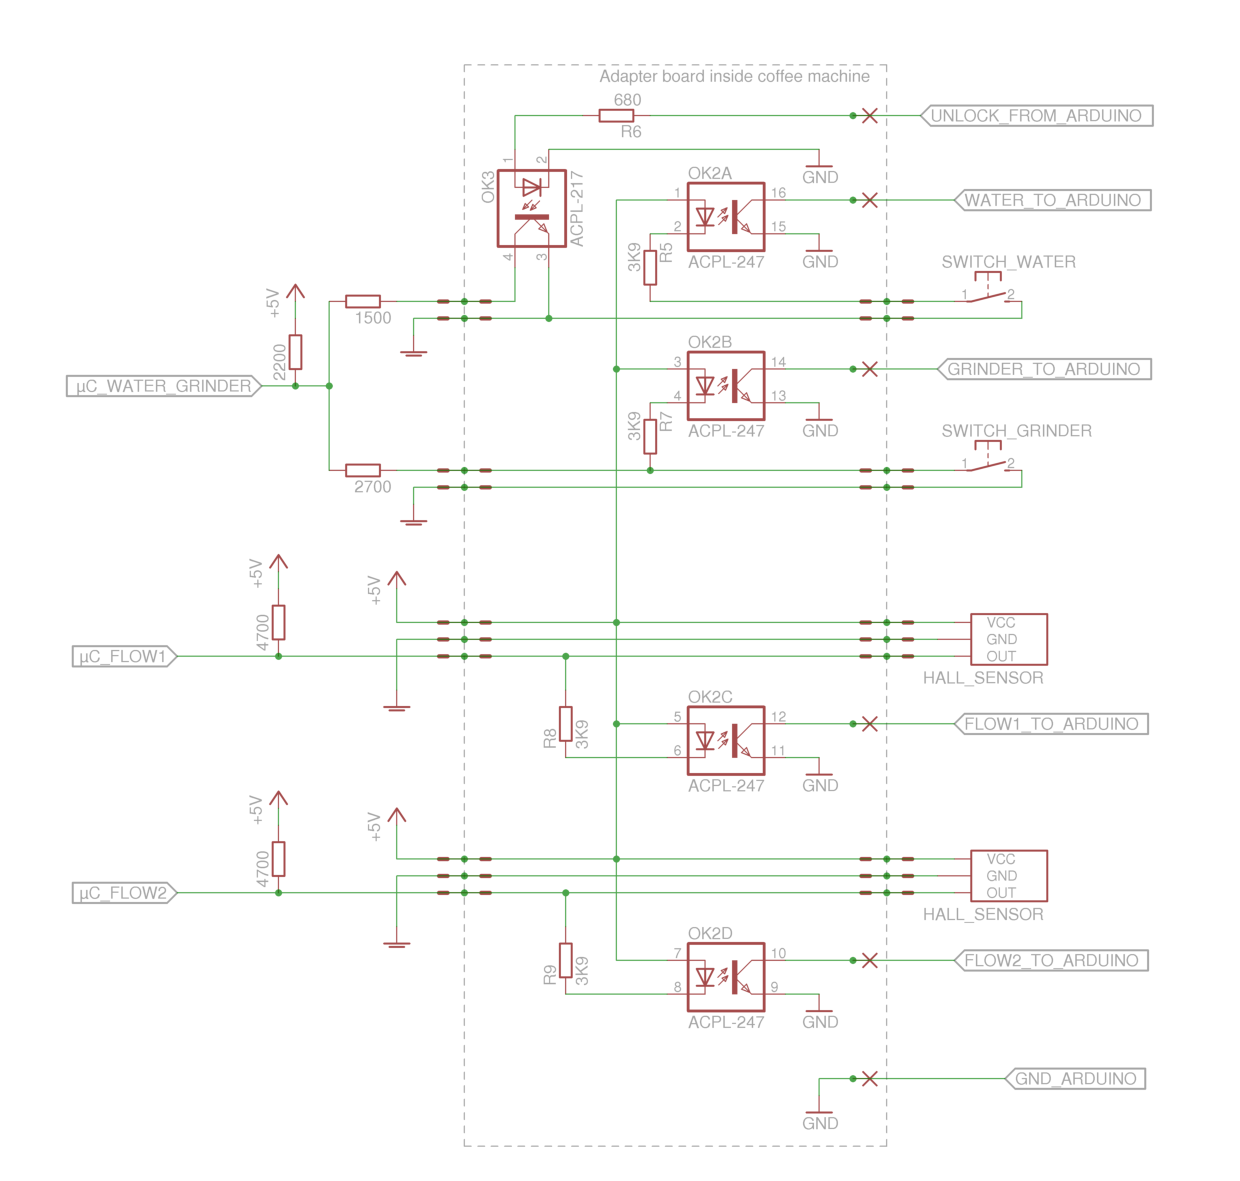
\includegraphics[width=17cm]{./images/oldPCBSchematic.pdf}
   \captionsetup{justification=centering}
   \caption{Schematic of the Adapter (taken from \cite{BachelorThesis})}
   \label{fig:pcb}
  \end{figure}
  \newpage
  \textbf{Adapter attached to the Raspberry Pi:}\\~\\
  The Raspberry Pi facing part will connected with wires to the board. The different connections can be viewed in figures \ref{fig:machinePins} \& \ref{fig:adapterraspberry} 
  
  \begin{figure}[H]
   \centering
   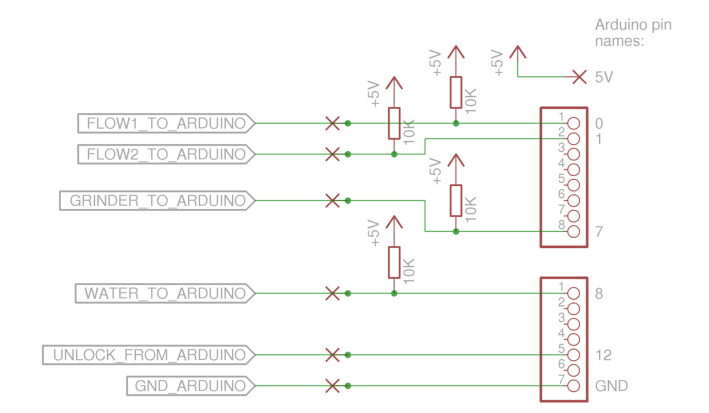
\includegraphics[width=10cm]{./images/adapterraspberry.pdf}
   \captionsetup{justification=centering}
   \caption{Adapter connected to the Raspberry Pi (taken from \cite{BachelorThesis})}
   \label{fig:adapterraspberry}
  \end{figure}
  \subsubsection{3D Case}
  
  In order to protect our system from physical damages, a custom 3D printed case was modelled. For this task, we used a high end 3D printer from Formlabs : Form 2.
  This printer uses a laser in order to solidify the resine and form the different layers.
   \begin{figure}[H]
   \centering
   \includegraphics[width=7cm]{./images/form2}
   \captionsetup{justification=centering}
   \caption{Formlabs: Form2 (Taken from \cite{formlabs})}
   \label{fig:form2}
  \end{figure}
  The model in Figure \ref{fig:model} was created using an open source software called Blender. The case is divided in 3 different pieces in order to fit the printer's build volume.
  The model will be then exported to the PreForm software to make the final adjustments before printing each part seperately. The average printing time for the each part is 15 Hours.
  
  \begin{figure}[H]
   \centering
   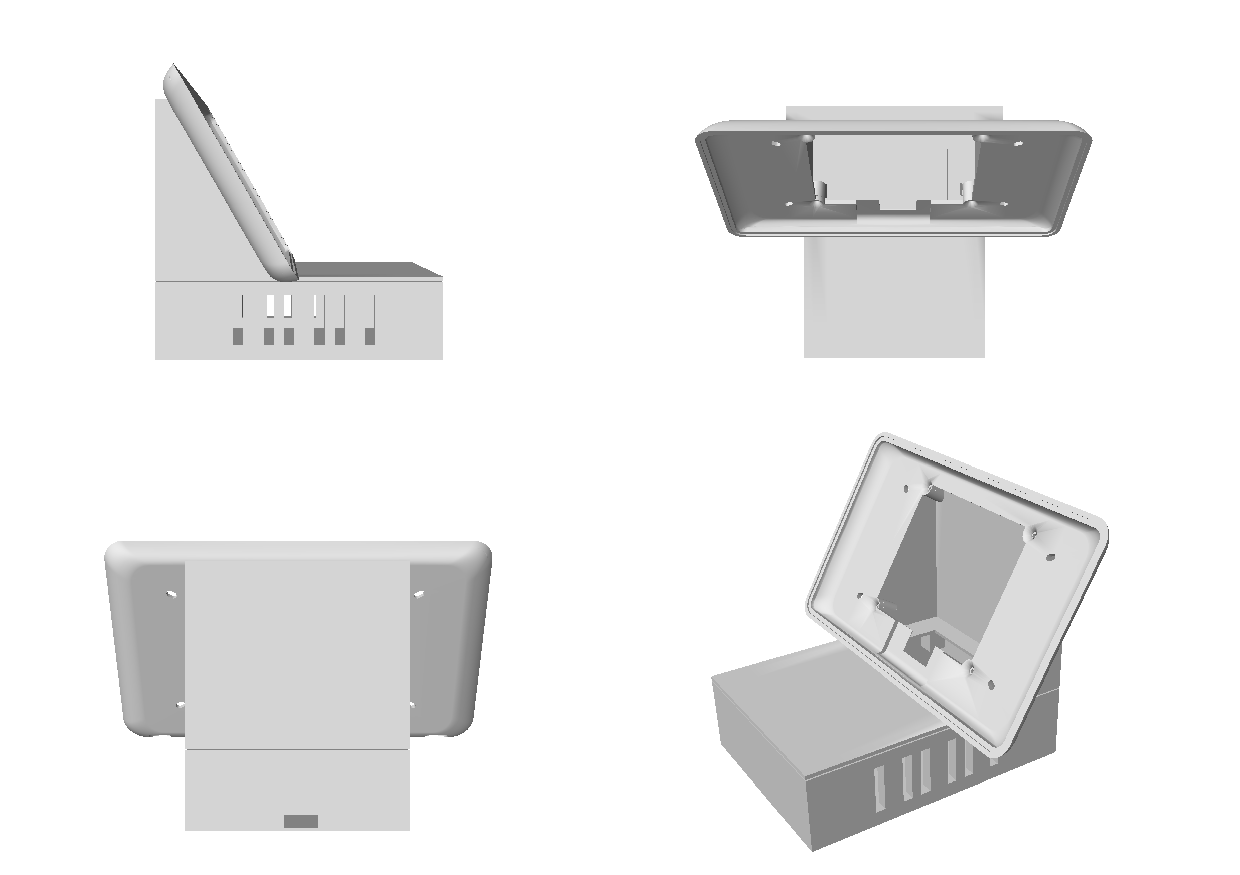
\includegraphics[width=1.0\textwidth]{./images/case}
   \captionsetup{justification=centering}
   \caption{3D Model Case}
   \label{fig:model}
  \end{figure}
  \subsection{Software}
  
  In order to provide a flawless user experience, we used state of the art technologies. Our system is divided in two main sub systems : Back-end and Front-end.\\~\\
  The Back-end manages the communication with the server, the off-line transactions, the monitoring system and downloading the entertainment material. \\~\\
  The Front-end is what the user interacts with : The Raspberry Pi's interface and Android interface as explained in section \ref{sec:raspberry} \& \ref{sec:android}. 
  Our main goal was to provide an interactive, intuitive and beautiful interface. 
  This part is implemented for the Raspberry Pi and Android Smartphones.\\~\\
  The main problem with the previous project was its complexity, and lack of portability.
  To tackle these problems and create an adaptive and extensible software, we divided our Back-end in two main parts :

   \begin{itemize}
    \item User interaction manager
    \item Monitoring and debugging system
   \end{itemize}
   
  \subsubsection{User interaction manager}
  
  The Raspberry Pi is the core of our system :
  \begin{itemize}
    \item It should be able to lock/unlock the coffee machine
    \item Manage the RFID input
    \item Communicate with the accounting system
    \item Provide entertainment content
    \item Intercept transactions from the android application
    \item Monitor the behaviour of the coffee machine
   \end{itemize}
   This part should be implemented in python. Due to thread scheduling problems in the Raspberry Pi,
   our system was divided in multiple subprocesses :
   \begin{itemize}
    \item Listening to incoming HTTP requests from the android application using the tornado library
    \item lock/unlock the coffee machine by simulating the water sensor signal
    \item Constantly listen to the RFID reader for any valid token
   \end{itemize}
   
   
   \textbf{UID detection :} \\
   
   The communication with the RFID-RC522 over SPI, is implemented using the python library MFRC522. The method read() in figure \ref{fig:rfidclass} verifies every 0.01 second the reader. 
   If a valid RFID emitter is detected and no user is already logged in, a custom QR code image containing the read UID is generated and the identifier is sent to the view class.
   If an android transaction was detected before the user put his card, the read UID is ignored and a message is displayed informing the user that the machine is already in use.\\
   
   \begin{figure}[h]
   \centering
   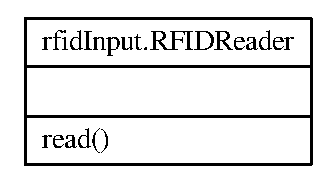
\includegraphics[width=5cm]{./images/rfidReaderClasses}
   \captionsetup{justification=centering}
   \caption{RFID class diagram}
   \label{fig:rfidclass}
  \end{figure}
  \textbf{Communication with the server :} \\
   
   In this project, we will use a preexisting accounting system to manage the transactions. After detecting the user's order, an HTTP request is sent to 
   \url{http://i80misc01.itec.kit.edu/coffee/buy.php?rfid=(1) &black=(2) &water=(3)}\\
   where (1) is the user's UID, (2) and (3) represent respectively the coffee and water choice. 
   If (2) is set to "true", the user doesn't want milk with his coffee.
   The prices are defined by the server.\\
   
   One other service provided by the server is getting user information. After launching a request to \url{http://i80misc01.itec.kit.edu/coffee/getuser.php?rfid=(1)}
   with (1) corresponding the the user's personal UID, a response with the user's name, token, and balance is returned from the server. The name and balance are displayed in the order page. 
   The token is used to display the user's personal transactions history in the accounting section. The different views will be analyzed in the User interface section.
   If the internet connection is missing, the system will use the local database for the transactions as explained in the Offline Handler section\\~\\
   \textbf{Offline Handler:}\\
   
   The standard behaviour of the system is to communicate with the server for each user's session.
   Unfortunately, this may not be always the case. The system is using a Mysql database as backup for these scenarios. 
   The coffee\_time database has two different tables as shown in figure \ref{fig:offlineDB}
   
    \begin{figure}[h]
   \centering
   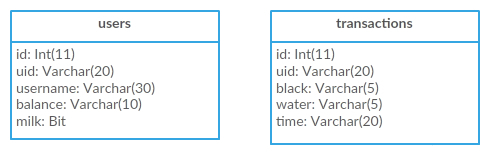
\includegraphics[width=10cm]{./images/offlineDB}
   \captionsetup{justification=centering}
   \caption{Tables used for the backup database}
   \label{fig:offlineDB}
   \end{figure}
  
  The users table contains the different required information about each user : UID, Name, and Balance. 
  On the other hand, the transactions table saves all offline transactions. For each order, the user's UID, the milk choice, water choice, and a time stamp are recorded in the database.
  Both tables are periodically updated by the system.\\~\\
  \textbf{Tornado Server:}\\
  
   One of the new implemented features in this system, is the possibility to order coffee from a smartphone. 
   For this purpose, the Raspberry Pi should be constantly listening for incoming HTTP requests using the tornado library.
   Tornado is an asynchronous networking library. It's an easy to learn Framework, that we used in order to intercept any incoming request from the android application.
   As depicted in figure \ref{fig:tornadoClass},
   the tornado class has two main methods: get() and post(). If a request is detected, the script verifies that no user is already connected. 
   If a user is already logged in, a warning message is sent via the post() method to the android application asking the user to retry after few minutes. 
   If the machine is free, the uid is sent to the RFID reading script where it will be processed as explained in the UID detection section.\\~\\
    \begin{figure}[H]
   \centering
   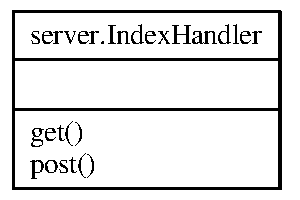
\includegraphics[width=4cm]{./images/tornadoServerClasses.pdf}
   \captionsetup{justification=centering}
   \caption{The tornado server class diagram}
   \label{fig:tornadoClass}
  \end{figure}
   \textbf{Locking mechanism:}\\
   
   In order to prevent unauthorized users from using the coffee machine, a locking mechanism was developed.
   The coffee machine provides serveral locking singals : Preventing the motor from going to brew position, stopping the grinder etc, but all these signals prevent only the coffee process.
   The best way to also prevent water usage, is to simulate the water level sensor. A low water will prevent any order from the coffee machine. 
   The only disadvantage of this mechanism, is the "Fill Water Tank" message displayed on the coffee machine, which can be misleading for some users.
   If the sensor is pulled down during a transaction, the coffee machine would think that there is enough water for another order, and stays unlocked.
   In order to prevent such unwanted behaviour, the coffee machine is locked at the end of the transaction regardless of the view locking.
   
  \subsubsection{Monitoring system}
  
  In this section, we will introduce a new feature implemented in this project : The Monitoring system. 
  The main role of this process is to manage the states of the whole program while logging all inputs from the coffee machine.
  For this purpose, we will use a python library named Transitions. This library is "A lightweight, object-oriented state machine implementation in Python"\cite{transitions}. \\~\\
  \textbf{Logging System:}\\~\\
  The logging system is in charge of parsing the coffee machine's input and delivering it to the state machine. The logging system is tuned by a config file.
  An example of such file can be viewed in listing \ref{lbl:config}.\\
 
  \begin{lstlisting}[caption={Example of config file for the logging system}, label={lbl:config}]
  
	    Gear switch home pos : 37, IN ; 35, IN
	    Gear switch brew pos : 33, IN; 31, IN
	    Hot water/ Steam switch : 29, IN
	    Brew unit : 40, IN
	    Dregs drawer : 38, IN
	    MS : 36, IN
	    Doser switch : 16, IN; 15, IN
	    Reed switch water level : 13, IN
	    Flow meter system 2 : 8, IN; 7, IN
	    Flow meter system 1 : 5, IN; 3, IN
	    
  \end{lstlisting}

  The general format of a config line would be as follows :\\ (Sensor's name) : (Pin 1 number), (Type : In/Out) ; (Pin 2 number), (Type : In/Out)\\
  When the logging system starts, the config file is read and parsed. The sensor names are stored in a List and printed at the beginning of the log file.
  The pins are stored next to each other starting from the first sensor's first pin. This list will be used to setup the GPIO pins according to their type (IN/OUT),
  and will be used in every iteration to read the inputs of every sensor, which will be stored in the log file with a timestamp as pictured in \ref{lbl:logfile}.
  With the oscilloscope, we could determine the frequency of the water flow sensors (100 Hz). This helped to determine the suitable reading frequency (1KHz).\\
  \begin{lstlisting}[caption={Example of a log file}, label={lbl:logfile}]
  
    [Gear switch home pos , Gear switch brew pos , 
	Hot water/ Steam switch , Brew unit , Dregs drawer,
	MS , Doser switch , Reed switch water level,
	    Flow meter system 2 , Flow meter system 1]
	
	14:39:56 [0,1,0,1,0,0,0,0,1,0,1,1,0,0,0,0]
	14:40:24 [0,1,0,1,0,0,0,0,1,0,1,1,0,0,0,1]
	14:40:25 [0,1,0,1,0,0,0,0,1,0,1,1,0,0,0,0]
	14:40:26 [0,1,0,1,0,0,0,0,1,0,1,1,0,1,0,0]
	14:40:27 [0,1,0,1,0,0,0,0,1,0,1,1,0,0,0,1]
	14:40:28 [0,1,0,1,0,0,0,0,1,0,1,1,0,0,0,0]
	
  \end{lstlisting}
  \textbf{State Machine:}\\~\\
  In order to provide a portable system, our FSM is dynamically generated. Therefore, the user will have to proceed as follows :
  \begin{itemize}
   \item Step 1 : The user creates a file for each state (water, coffee, etc). Each file's name corresponds to the state's name.
   \item Step 2 : The user copies then the logs corresponding to each action (Order coffee, order water, etc) from the log file to each file created in the previous step
  \end{itemize}

  The code snippet \ref{lbl:waterState} represents the current water state file. Each line corresponds to an input from the coffee machine, where every number is the state of the different sensors.
  When stating our application, the system will read the different states and generate the corresponding Finite State Machine. 
  If a new input is detected, the system will move to the unkown state.
  All inputs in this state will be written to a new file. As soon as the idle input is detected, the system will change to the idle state. 
  The user can then lable the new generated file with the corresponding state, which will be added the the FSM after restarting the application.\\
  \newpage
   \begin{lstlisting}[caption={Sample of the water state file}, label={lbl:waterState}]
   
		  0,1,0,1,0,0,0,0,1,0,0,0,0,0,0
		  0,1,0,1,0,0,0,0,1,0,0,0,1,0,1
		  0,1,0,1,0,0,0,0,1,0,0,0,0,0,0
		  0,1,0,1,0,0,0,0,1,0,0,0,0,0,1
		  0,1,0,1,0,0,0,0,1,0,0,0,0,0,0
		  0,1,0,1,0,0,0,0,1,0,0,0,1,0,0
		  0,1,0,1,0,0,0,0,1,0,0,0,0,0,1
		  0,1,0,1,0,0,0,0,1,0,0,0,1,0,0
		  0,1,0,1,0,0,0,0,1,0,0,0,1,0,1
		  
  \end{lstlisting}
   As shown in figure \ref{fig:stateMachine}, our State Machine can be divided in 5 different states : Idle state, coffee state, water state, no water state, unkown state.
  The current state is defined by the coffee machine. \\~\\
  After the FSM is generated, every output from the coffee machine is converted to a function's name using the convertToFunc method. 
  The next step is to call the method in the state machine's instance. Depending on the input, the FSM will move to the corresponding state.
  If an uncommon input is detected, the FSM moves to the unkown state as shown in listing \ref{lbl:fsmCall}.\\
   \begin{lstlisting} [caption={FSM call code snippet}, label={lbl:fsmCall}]
   try:
       moveToState = getattr(coffeeMachine, 
                          coffeeMachine.convertToFunc(s))
       moveToState()
   except AttributeError as e:
       print(str(e))
   except MachineError :
       coffeeMachine.toUnkown()
  \end{lstlisting}
  
   \begin{figure}[H]
   \centering
   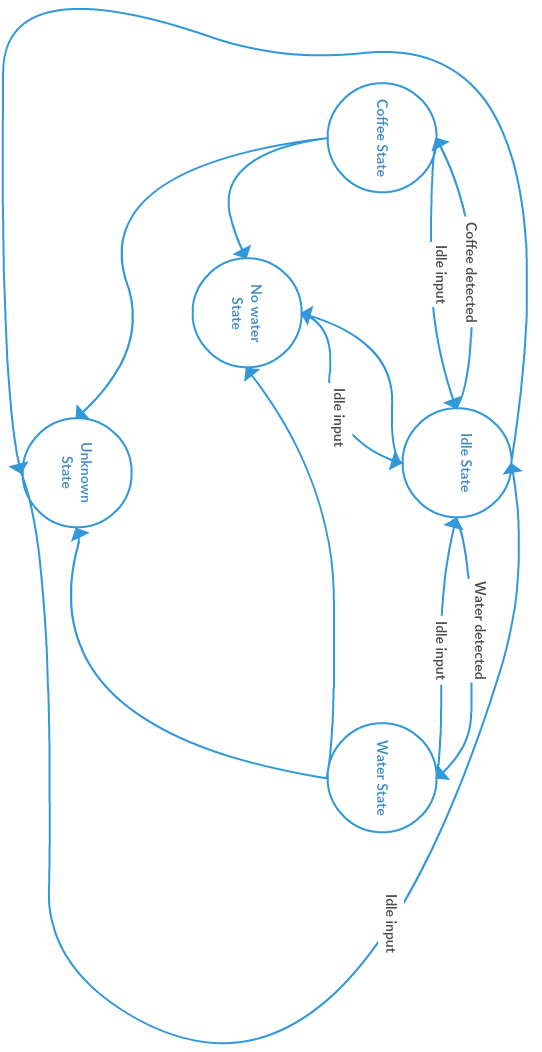
\includegraphics[height=1.0\textheight]{./images/stateMachine}
   \captionsetup{justification=centering}
   \caption{The State Machine graph}
   \label{fig:stateMachine}
  \end{figure}
  
   Before or after state transition, a custom method is called as pictured in \ref{fig:stateMachineClass}.
  Depending on the current state, the FSM has to ensure the corresponding behaviour.
  In the idle state, the coffee machine has to remain locked, and the RFID reading script is continuously called.
  When a valid card is detected, the coffee machine is unlocked, and the RFID reading script is paused.
  If a coffee/water input is detected, the FSM moves to the corresponding state, saving the order in a list. 
  When the coffee machine enters the idle state for longer than 3 seconds, the system sets the "done" flag to True and the corresponding transaction is transmitted to the server.\\
  
  The unkown state or the noWater state can be accessed from any other state. In order to leave the unkown state, the coffee machine has to send the corresponding idle output.
  When the water tank is refilled, the FSM will be back to the idle state.\\
  
  The problem with the dynamic approach is that it's a little bit slow compared to the logging rate. A hard coded version of all the states was implemented in order to avoid such latency.\\
  During the different states, the logging system will write the input with a timestamp to a file if the new value differs from the previous one.
  This ensures a compressed log of the daily behaviour.
  Everyday at midnight, a new file is created with the corresponding date to contain the daily logs, and a cleaning script is started. 
  The main role of this script is to ensure that a log file is not saved for longer than a week.\\
  
  \begin{figure}[H]
   \centering
   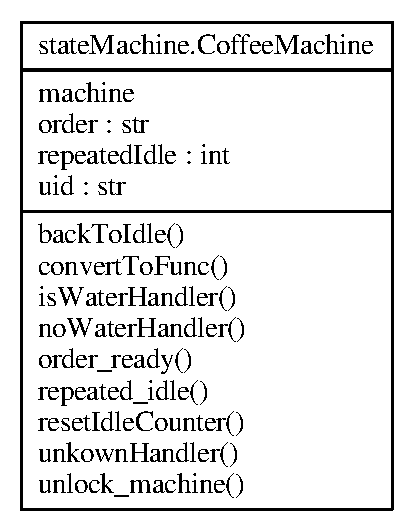
\includegraphics[width=6cm]{./images/stateMachineClasses.pdf}
   \captionsetup{justification=centering}
   \caption{The State Machine class}
   \label{fig:stateMachineClass}
  \end{figure}
  
  \subsubsection{Raspberry pi Interface} \label{sec:raspberry}
   
   Our Front-end is divided in two main interfaces.
   The Raspberry Pi's interface is the main view used for interaction with the coffee machine. 
   It should provide a responsive user interface and manage the communications between the different subprocesses.
   This is the core of our system, and therefore it should be carefully architected. In order to 
   provide a robust system, 
   we will use the python library PyQT for the different views and threads management.
   The architetural pattern used is the model-view-controller pattern. 
   Each View has a corresponding controller, which will intercept the user's input, and make the corresponding changes in the model.
   
   \begin{figure}[H]
   \centering
   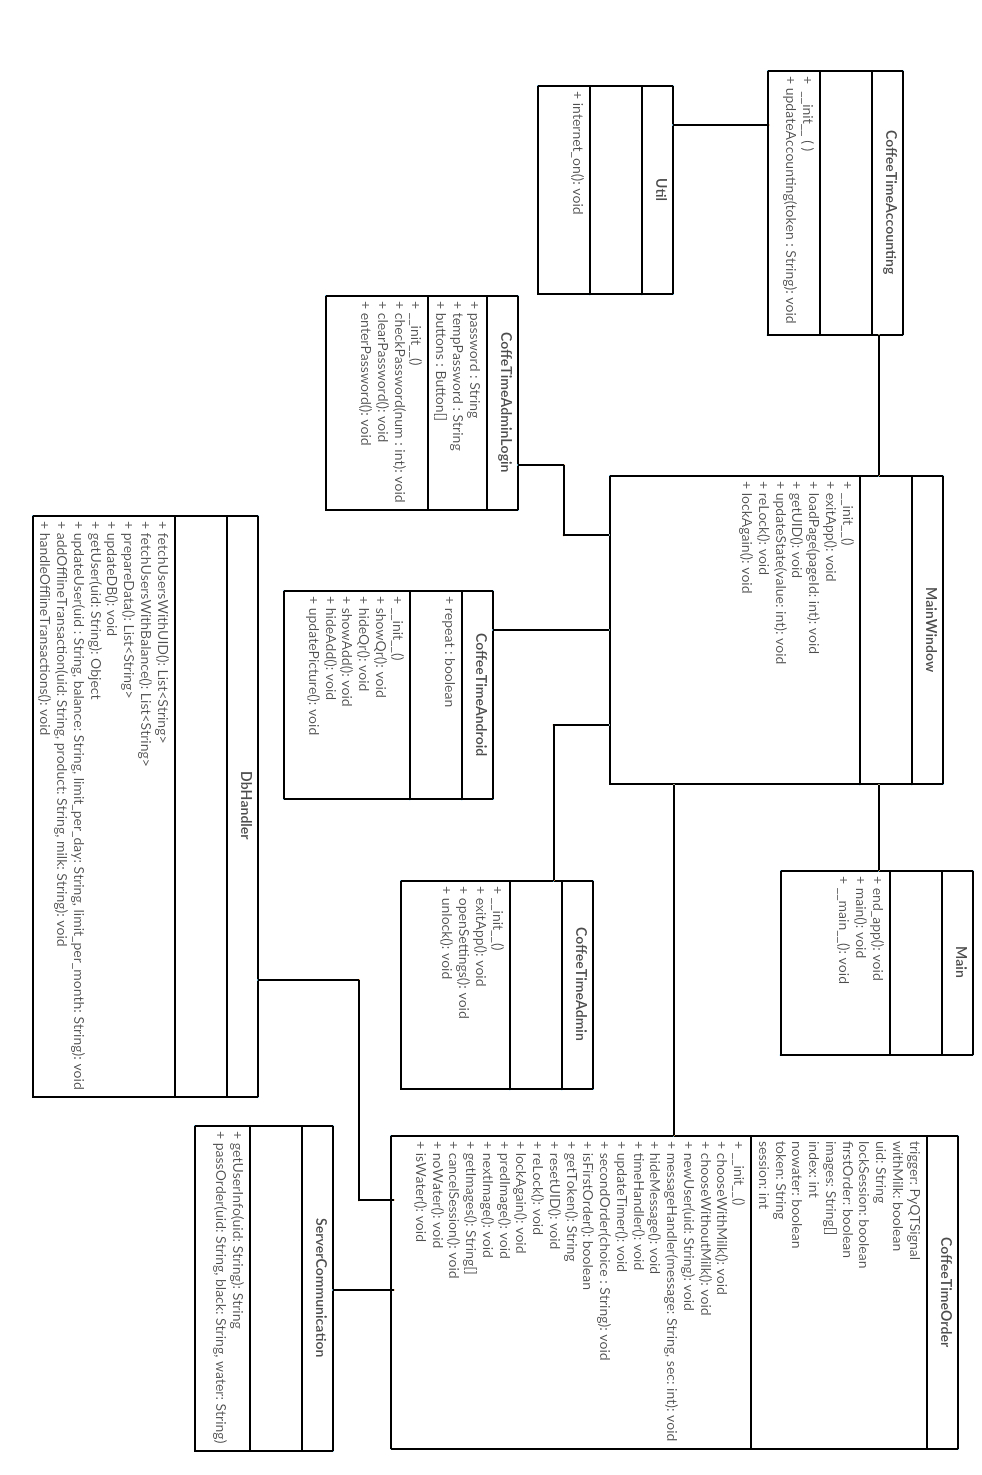
\includegraphics[width= 15cm]{./images/viewsClasses}
   \captionsetup{justification=centering}
   \caption{Class diagram of the user interface}
   \label{fig:viewsclasses}
  \end{figure}
  
   Our interface is divided in 4 different pages. In the main page (see figure \ref{fig:orderPage}), the user has the possibility to view his balance, and
   choose if he wants milk with his coffee. This choice will be saved as preference and displayed for his next order (The user has the possibility to change it). \\
   \begin{figure}[h]
   \centering
   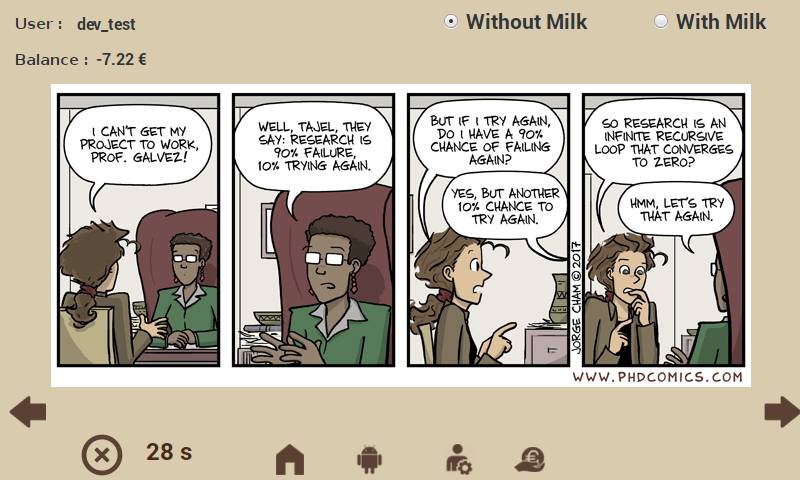
\includegraphics[width=1.0\textwidth]{./images/order_page}
   \captionsetup{justification=centering}
   \caption{The ordering page}
   \label{fig:orderPage}
  \end{figure}
  
   The server offers daily new entertainment content which can be accessed under \url{http://i80misc01.itec.kit.edu/cybercoffee_entertainment/linklist}.\\
   A python script is triggered everyday at 7 A.M to access the link above, parse it's content, get the respective links for the different images and download them. 
   The downloaded pictures can be viewed in the main page, or in the saving screen. Images are saved up to 2 weeks then deleted.
   Due to the pictures's high resolution, every image is scaled to the screen's hight or width depending on its dimensions.
   The class reponsible for the entertainment content is the downloadPictures as shown in figure \ref{fig:downloadPictures}. 
   The method getLinks returns a list with the different links to each image as explained previously. The method makeSpace, is triggered when the script is started. 
   It will look for files older than two weeks and delete them.
   Due to the lack of file extension in the links, the library BeautifulSoup is used to find the corresponding type of each image.
   All the downloaded pictures are stored under the Pictures folder, where they can be accessed by the view class or the screen saver.\\
   \begin{figure}[H]
   \centering
   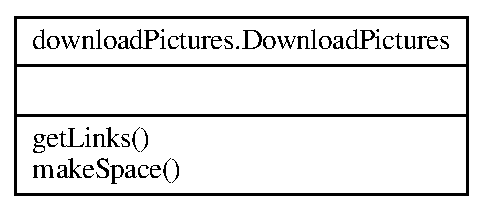
\includegraphics[width=7cm]{./images/entertainmentClasses}
   \captionsetup{justification=centering}
   \caption{The entertainment manager class}
   \label{fig:downloadPictures}
  \end{figure}
    
   The second window is the app center. As pictured in figure \ref{fig:android_page}, the user can either download the app by pressing the download button and scanning the given QR code, 
   or add his UID to the android app. This can be done by placing the RFID identifier and scanning the generated QR code after pressing the "Add User" button.\\
   \begin{figure}[H]
   \centering
   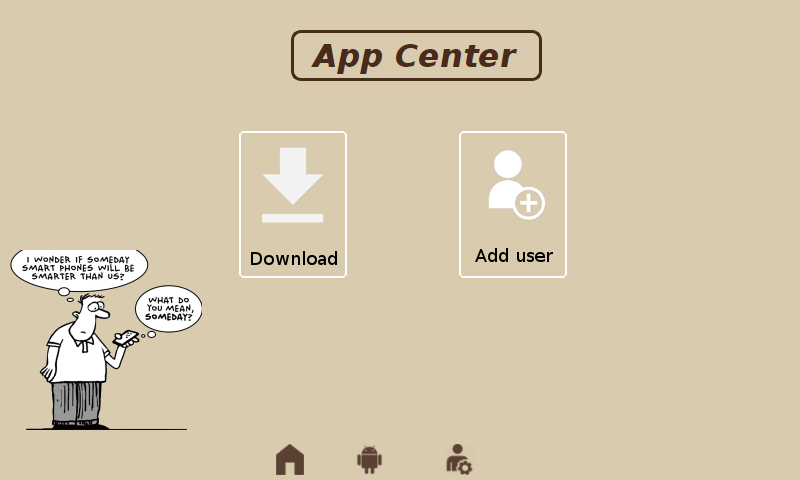
\includegraphics[width=1.0\textwidth]{./images/android_page}
   \captionsetup{justification=centering}
   \caption{The App center page}
   \label{fig:android_page}
  \end{figure}
  
   The accounting page, provides an up-to-date statement of all accounts. This page is updated after each transaction.
   It can be viewd under \url{http://i80misc01.ira.uka.de/coffee/kasse.php?token=C0FFE}\\
   
   The last page, is the admin page. This section is password protected. 
   After entering the right combination, the user has the possibility to unlock the coffee machine (for maintenance), enable/disable ssh connections, or exit the application.\\~\\

   \subsubsection{Android Application} \label{sec:android}
  
   After downloading the application from the server, the user is presented with a welcome screen(Figure \ref{fig:android-login-page}) where he can scan his UID.
   This window is presented only the first time the user opens the application.\\
   \begin{figure}[H]
    \centering
    \begin{subfigure}{.5\textwidth}
      \centering
      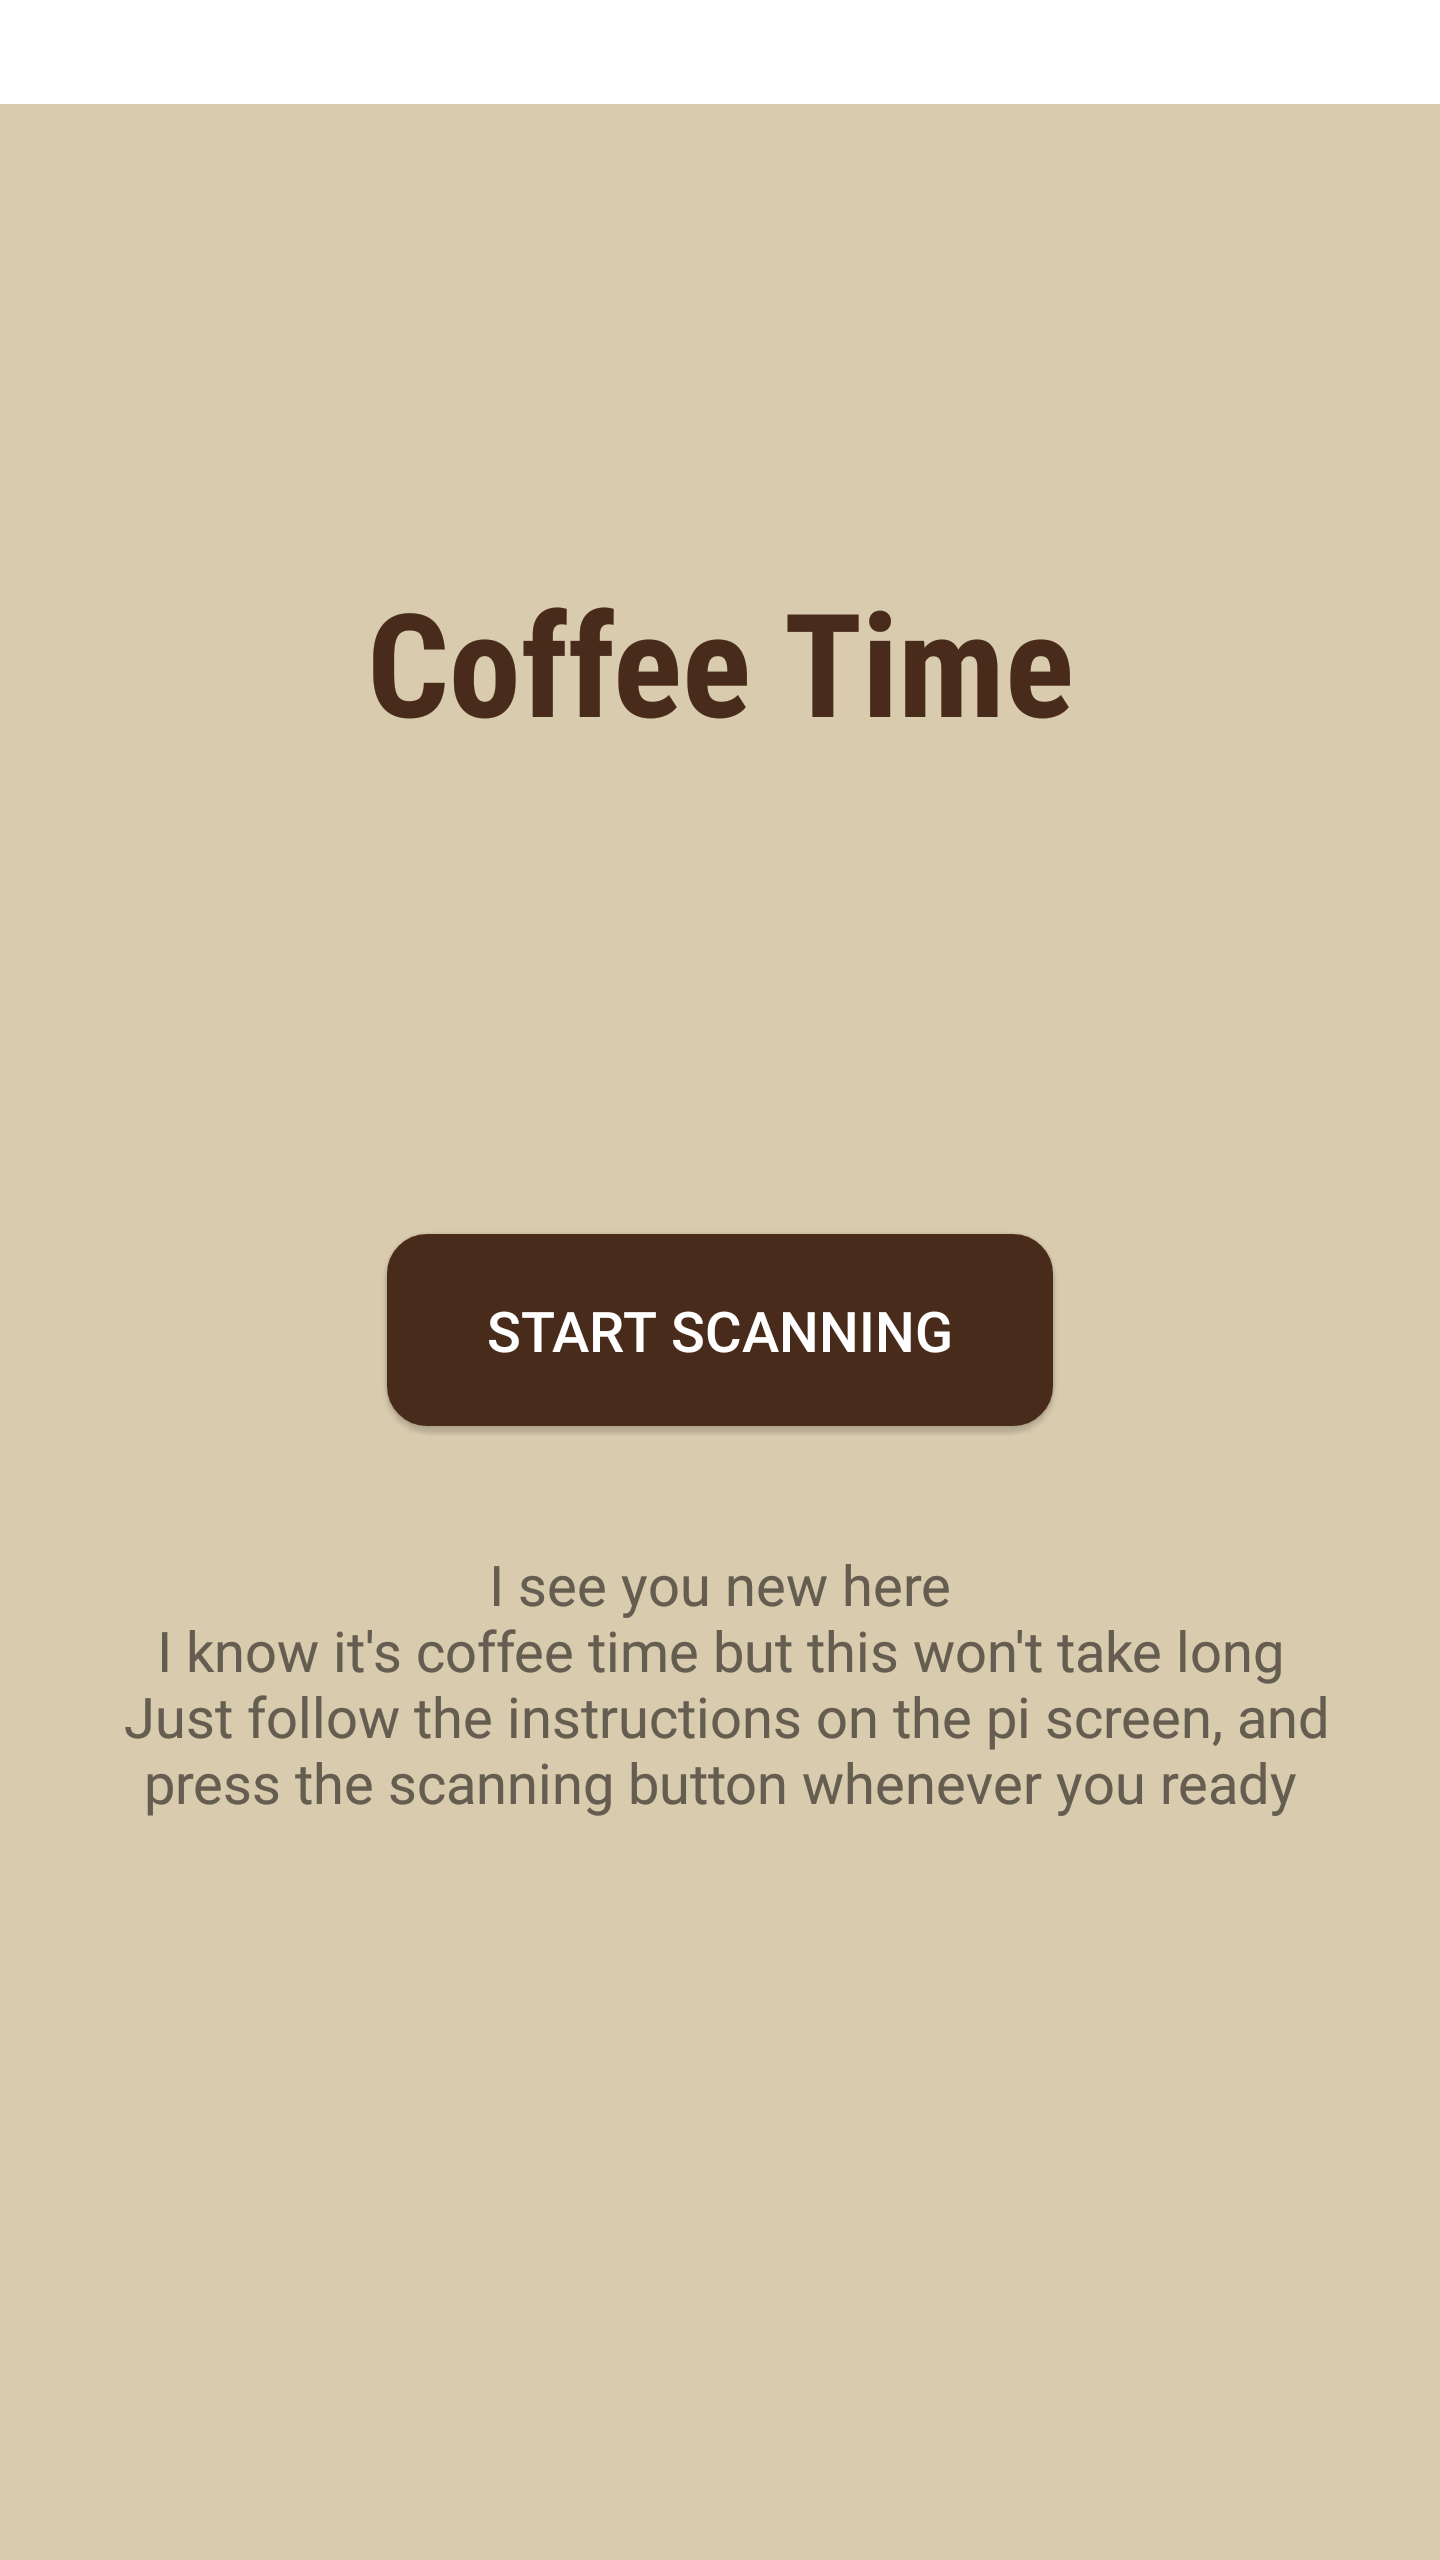
\includegraphics[width=.4\linewidth]{./images/android-login}
      \caption{Android login page}
      \label{fig:android-login-page}
    \end{subfigure}%
    \begin{subfigure}{.5\textwidth}
      \centering
      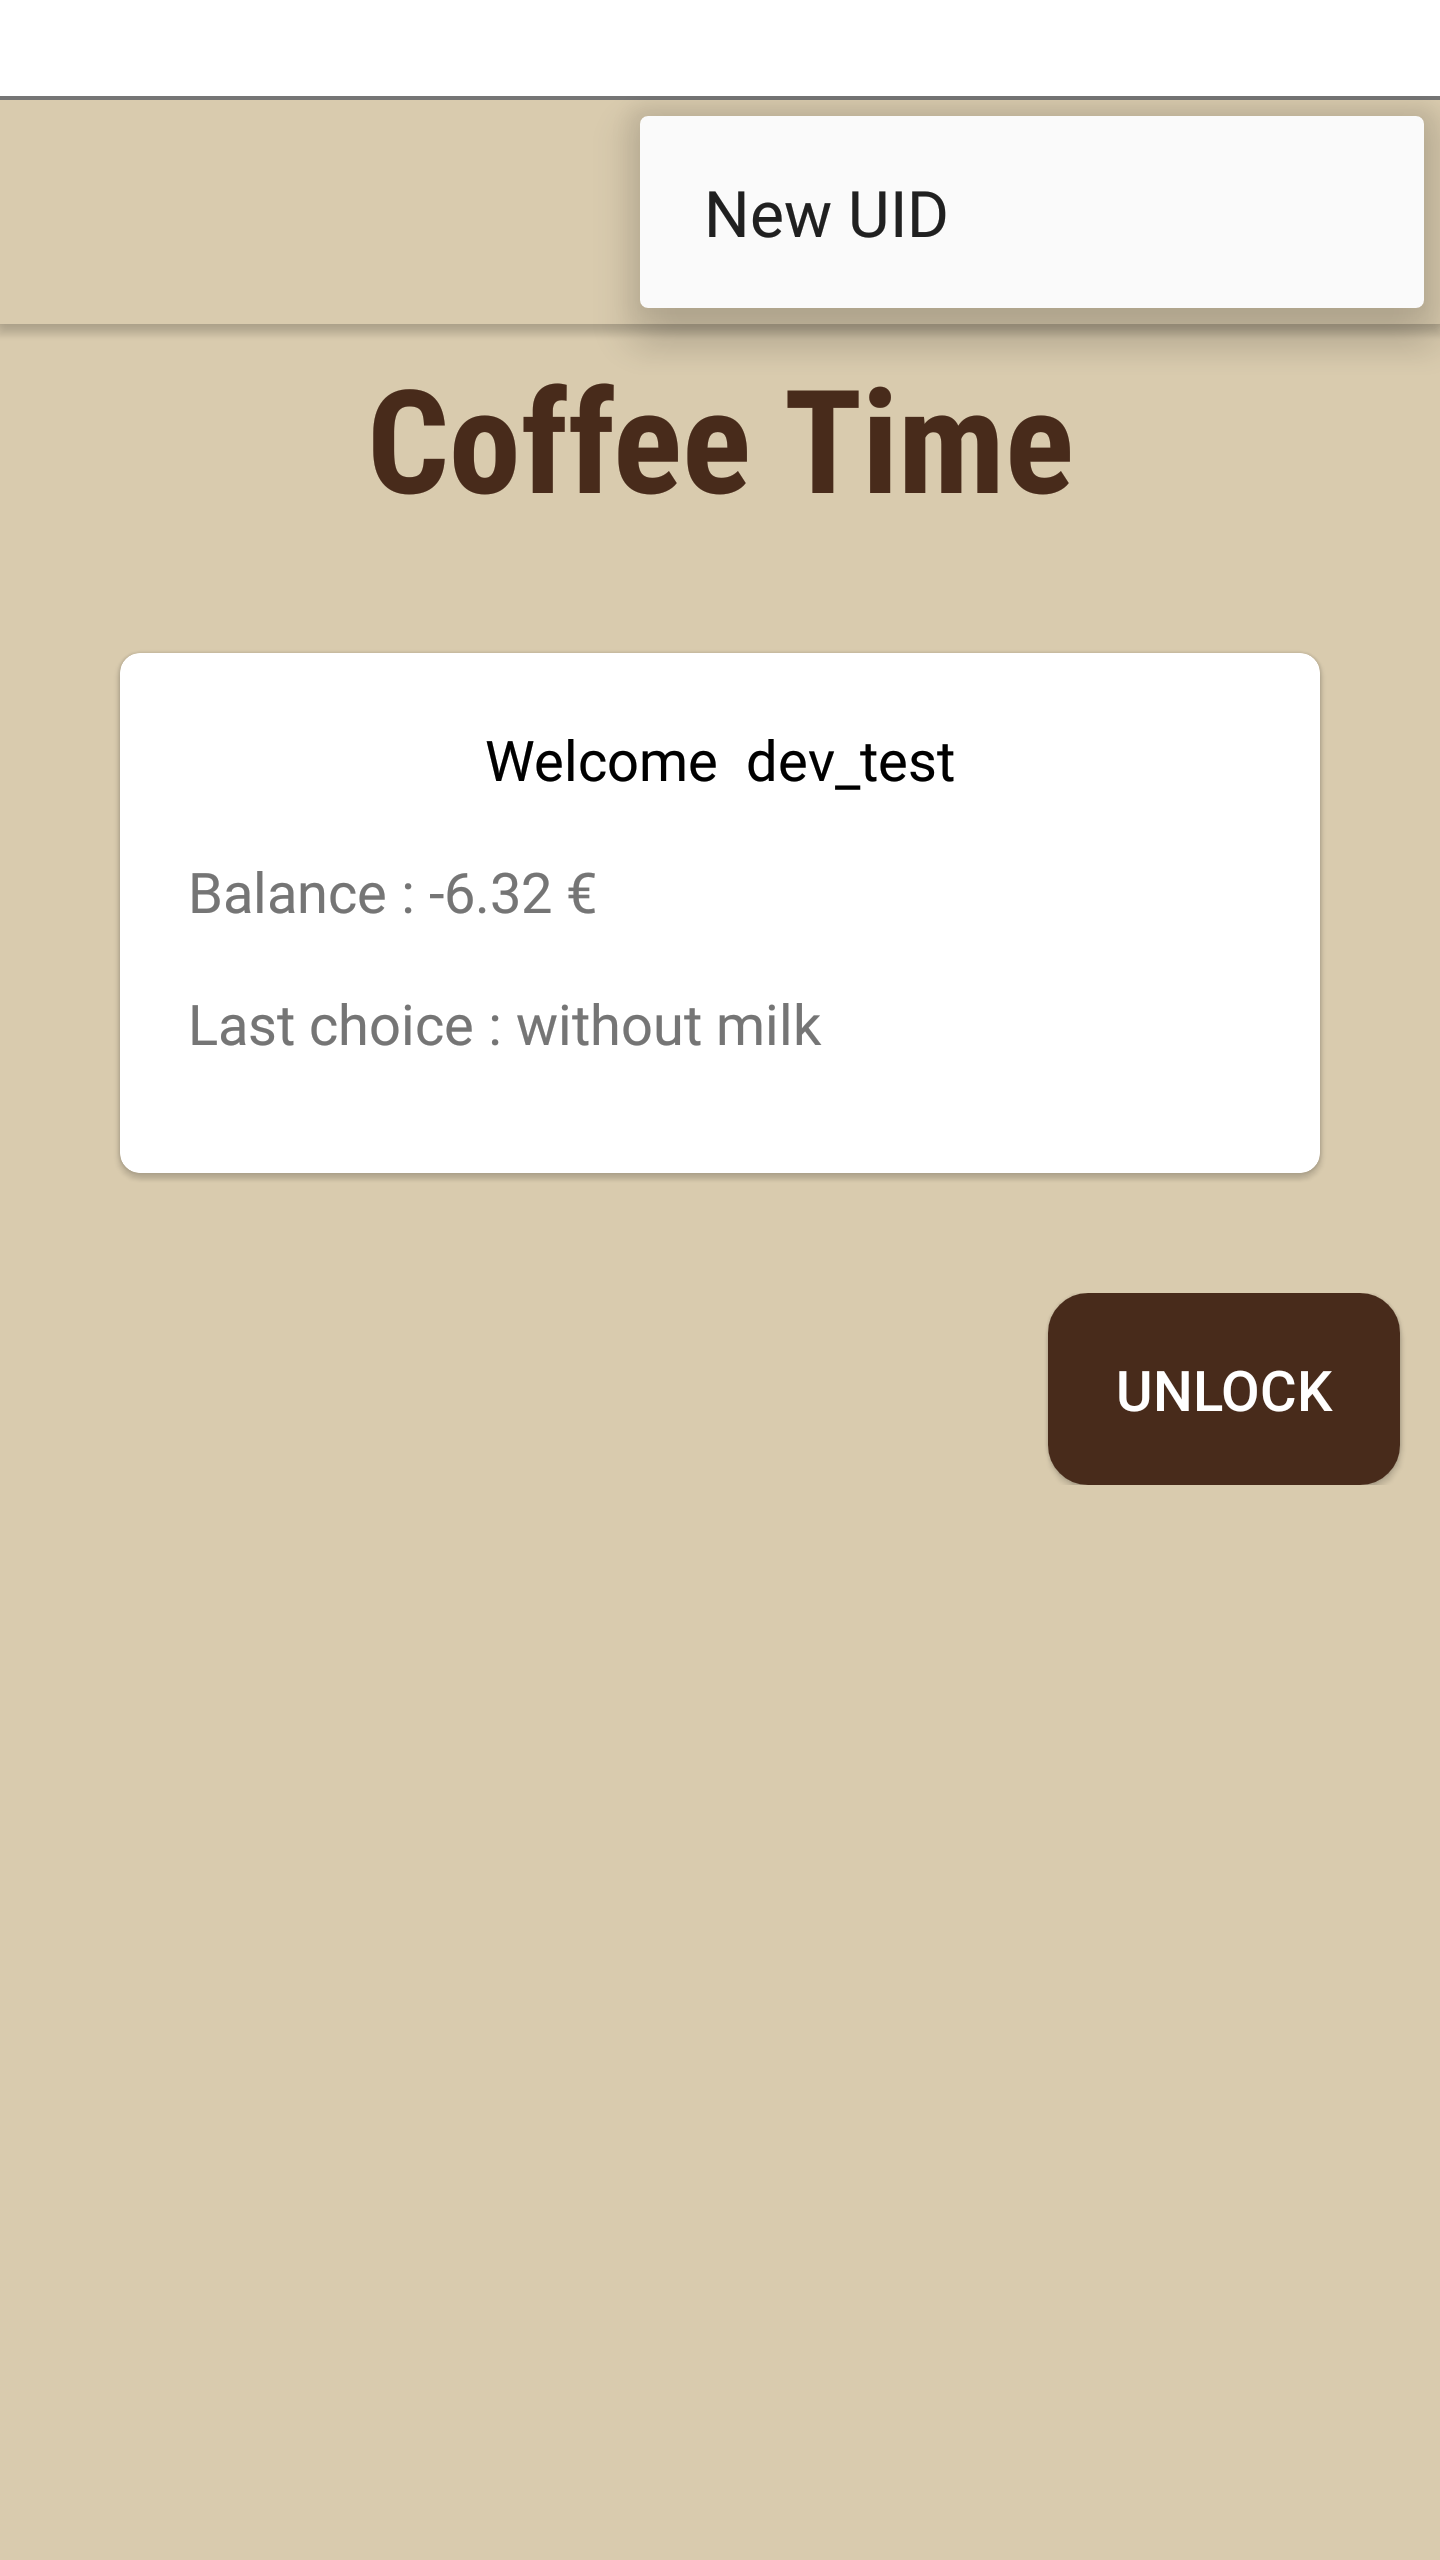
\includegraphics[width=.4\linewidth]{./images/android-main}
      \caption{Android main page}
      \label{fig:android-main-page}
    \end{subfigure}
    \caption{Android application windows}
    \label{fig:android-windows}
   \end{figure}
   
   When accessing the main window, the user can consult his balance, and unlock the coffee machine from distance. 
   If the user changed his physical RFID, he can update his new UID by pressing the New UID button (Figure \ref{fig:android-main-page}).\\
   This feature opens new possibilities : Offering coffee points to a friend as a gift etc
  
  \subsubsection{Communication between processes}
  
  The python language can't manage threads concurrently. One way to solve this problem was to divide the program in different subprocesses working concurrently.
  The problem we faced was the communication between the different processes. Possible solutions:
  \begin{itemize}
   \item Shared memory : Didn't work on the Raspberry Pi
   \item Pipes : Due to the different processes cycles, this solution was slowing the system
   \item Sockets : Blocking solutions will stop the system
   \item Simple text files : This simple solution is currently used
  \end{itemize}
  
  The different processes communicate by creating a file and name it according to the desired flag : Nowater, done, etc. 
  The different processes verify if the file exists and operate accordingly. 
  Some files may contain useful information : Order (contains the user's order), UID (contains the user's UID).
  A general overview of the communication mechanism can be viewed in figure \ref{fig:communication}.
  For example : When a user presents a valid RFID Token, the RFID reader process generates a file named uid.txt containing the user's uid along with userUID.png (QR Code containing the uid).
  This file is detected by the controller, which will ask the server for the user's name and balance using the read uid. The server's response is sent to the view, and the uid file is deleted.
  The userUID will be deleted after the session is over (30sec, or order detected).
  \begin{figure}[H]
   \centering
   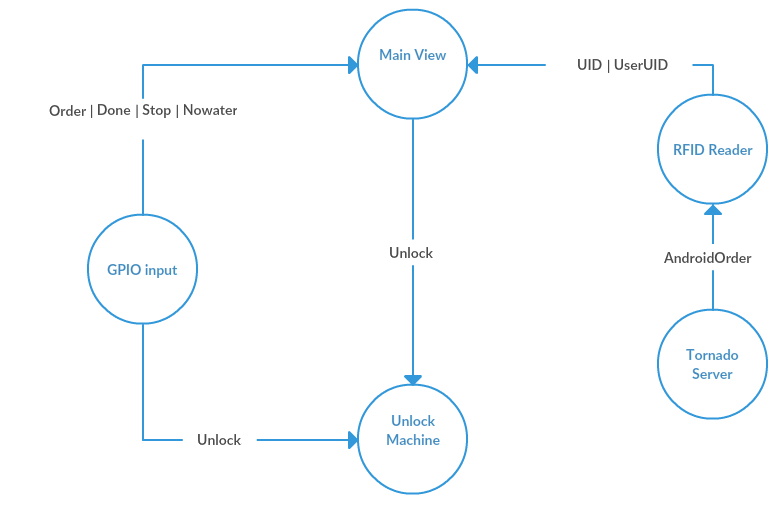
\includegraphics[width=7cm]{./images/communication.pdf}
   \captionsetup{justification=centering}
   \caption{Communication between the different processes}
   \label{fig:communication}
  \end{figure}
  
  \subsection{Challenges}
  
  In this section, we will discuss the different problems we encountered during this upgrade.
  One of the main difficulties we experienced was a variant output from the coffee machine. The idle state would be different from day to day. 
  This was caused by bad connections with the PCB. The problem was solved after the installation of the final pcb and increasing the reading Frequency ( From 100Hz to 1kHz).\\
  
  The main difference between the previous setup and this new upgrade is the number of devices managing the system. 
  Due the different processes running concurrently with high frequencies, we encountered random misbehaviours. 
  A custom scheduler was developed to improve the response time and reduce the chances of having two high priority jobs processed at the same time. 
  This improved the responsiveness of the system, providing a better user experience.\\
  
  Another reported problem was the RFID reader not responding or has a long response time.
  The issue could be hardware related (Faulty cable etc), or software related.
  We first isolated the Hardware possibility by replacing the cables and testing the components seperately. 
  Concluding that the problem wasn't hardware related, we started the reading code in a seperate script with higher CPU priority.
  Due to the uncommonness of this problem, this solution is still not confirmed. If the problem persists, a radical action may be taken such as automatic reboot.\\
  
  
  %The android application was designed to send requests to the Raspberry Pi using HTTP requests, the problem we encountred was that the Firewall would block any traffic.
  %One idea was to write a PHP script on the server's side that would fetch the HTTP request from the Android application and forward it to the Raspberry Pi.
  %Unfortunately, this method didn't work.
  %In order to improve the user experience and provide a faster response time, 
  %the suboptimal techniques used for the communication between the different processes were replaced by more complex and efficient methods.
  %Each file was replaced by a flag in the shared memory.
  %In order to prevent undesirable behaviour, semaphore is used to ensure that a value can be accessed by only one process at a time.
  \subsection{Costs}
  
  The different hardware parts cost 138,92 \euro as mentioned in detail in Table \ref{tab:cost}.\\~\\
  
  \begin{table}[H]
  \centering
  \begin{tabular}{llr}
   \hline
  \multicolumn{2}{c}{Item} \\
  \cline{1-2}
  Component & Description & Price(\euro) \\
  \hline
  Raspberry pi 3 & Model B & 33,61 \\
  Touchscreen & LCD touch display 7\,'' & 67,22 \\
  RFID Reader & Joy-IT RFID Module MFRC-522 & 8,39 \\
  Netzteil & & 10,92 \\
  \hline
  Total  & & 138,92 \\
  \hline
  \label{tab:cost}
  \end{tabular}
  \caption{Costs of the different Hardware parts}
  \label{tab:cost}
  \end{table}
  
  The other cost that must be taken under consideration is the power consumption.
  According to \cite{powerConsumption} a Raspberry Pi 3 consumes around 3W in our case. The value of the kWh is around 0.2916 \euro as mentioned by \cite{BDEW}
  This leads to a total cost of 7.47 \euro per year.
  
  \pagebreak
 
  \pagebreak
  \section{Conclusion}
  The system created during this thesis was developed in order to tackle few problems observed while using an off-the-shelf coffee machine in a common space:
  \begin{itemize}
   \item Prevent unauthorized users from using the coffee machine
   \item Endless counting of tally sheets
   \item Ordering without having a positive balance
  \end{itemize}
  The new system helps the coffee administrator by providing a secure and immediate connection between the user and the accounting system.
  This prevents endless tally sheets counting and accounts having a negative balance, plus no user can pretend forgetting to write his order. 
  The upgrade provides :
  \begin{itemize}
   \item A decent authentication mechanism using RFID tokens, preventing unauthorized users from using the coffee machine.
   \item The possibility to use a smartphone as an authentication device
   \item Daily entertainment content
   \item Automated order detection mechanism, which charges the user accordingly
  \end{itemize}
  
  In this thesis, we used the coffee machine's pins as a way to determine the machine's current state.
  A better approach would be to control the coffee machine directly, this would prevent any unwanted behaviour. 
  A sound based detection system could ensure better results than the sensor's input, providing a better overview of the system.
  \pagebreak
   \clearpage
\begingroup
  \pagestyle{empty}
  \null
  \newpage
\endgroup
  
%------------------------- Literaturverzeichnis ---------------------------- 
  \bibliographystyle{alpha}
  \bibliography{sample}
  
    \pagebreak
   \clearpage
\begingroup
  \pagestyle{empty}
  \null
  \newpage
\endgroup
  
  \appendix
  \section{Appendix}
  \subsection{The new PCB : Design}
   \begin{figure}[H]
   \centering
   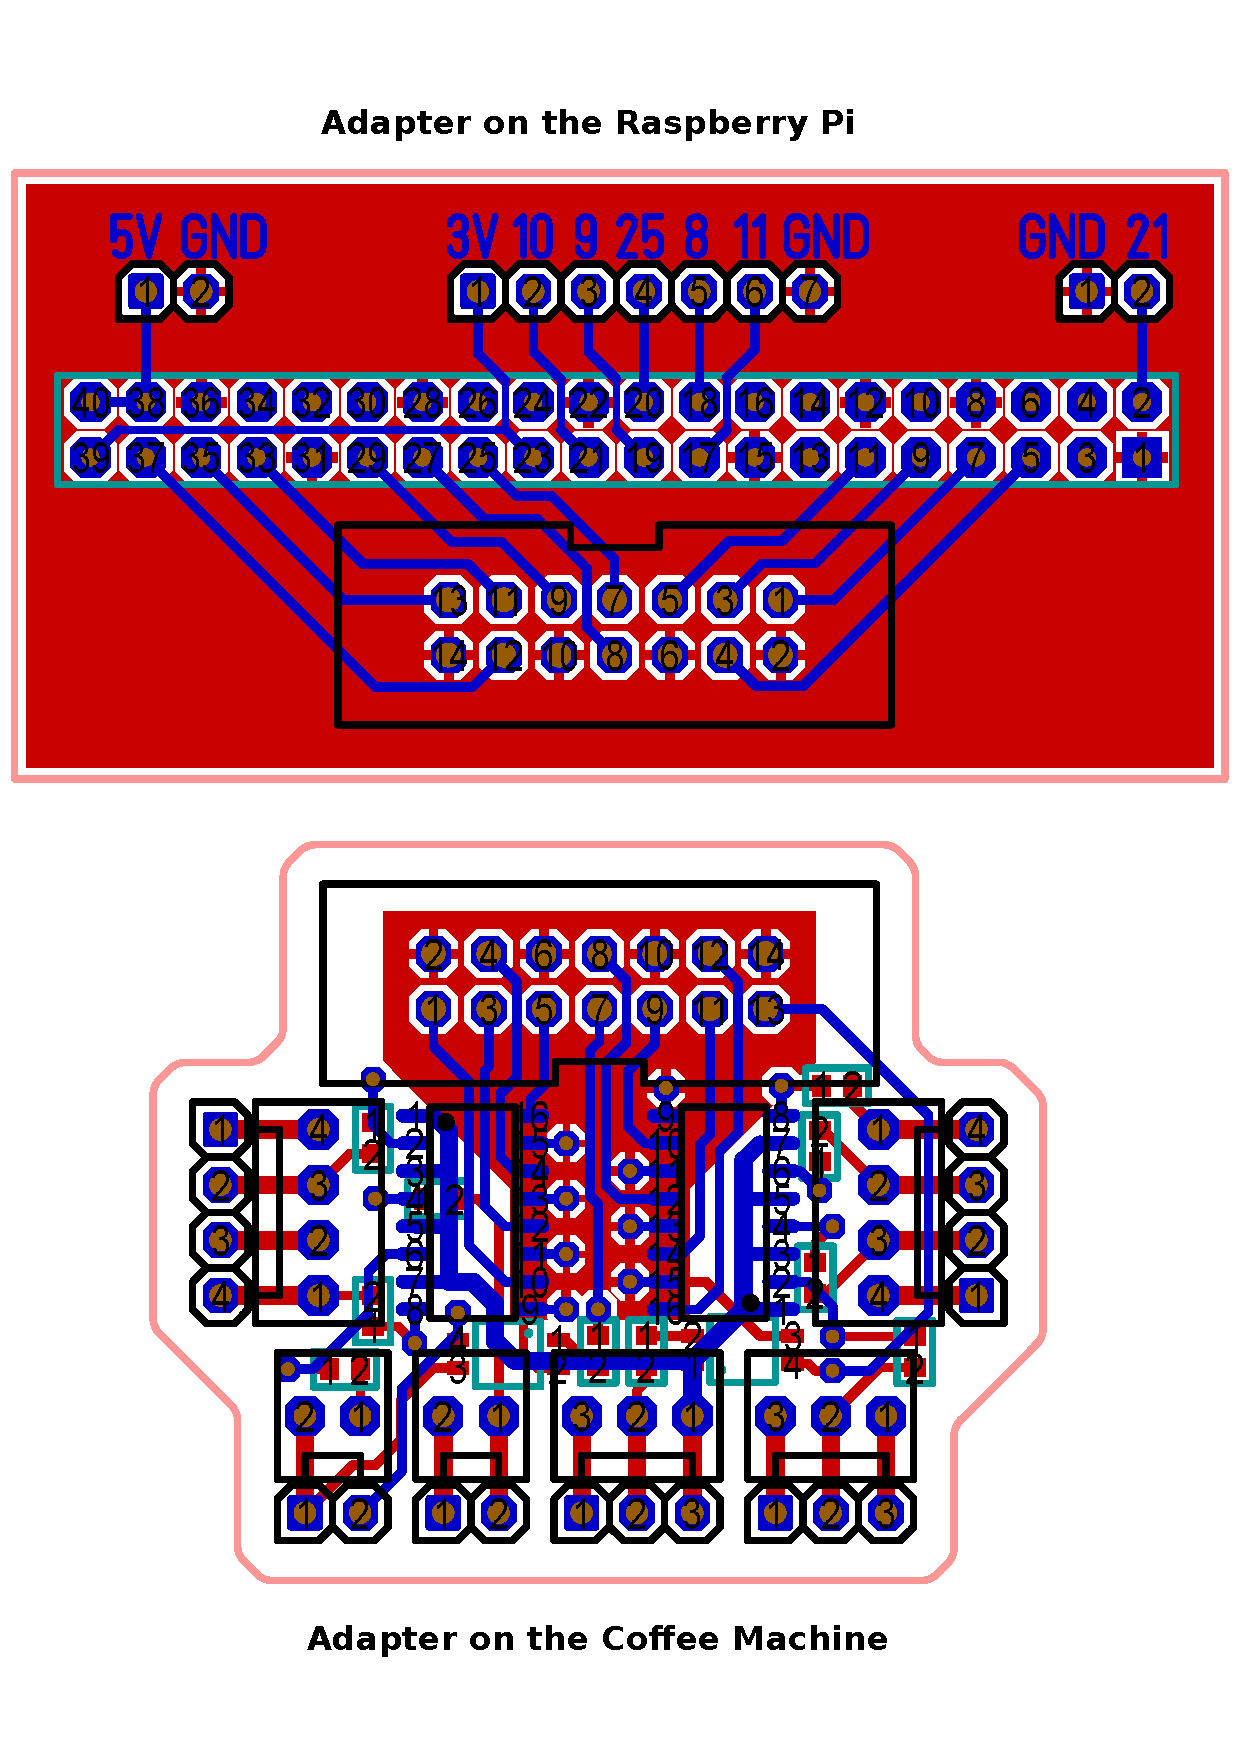
\includegraphics[width=15cm]{./images/pcb.pdf}
   \captionsetup{justification=centering}
   \caption{Adapter Coffee machine/ Raspberry Pi}
   \label{fig:newPCBDesign}
  \end{figure}
  \subsection{The new PCB : Schematic}
   \begin{figure}[H]
   \centering
   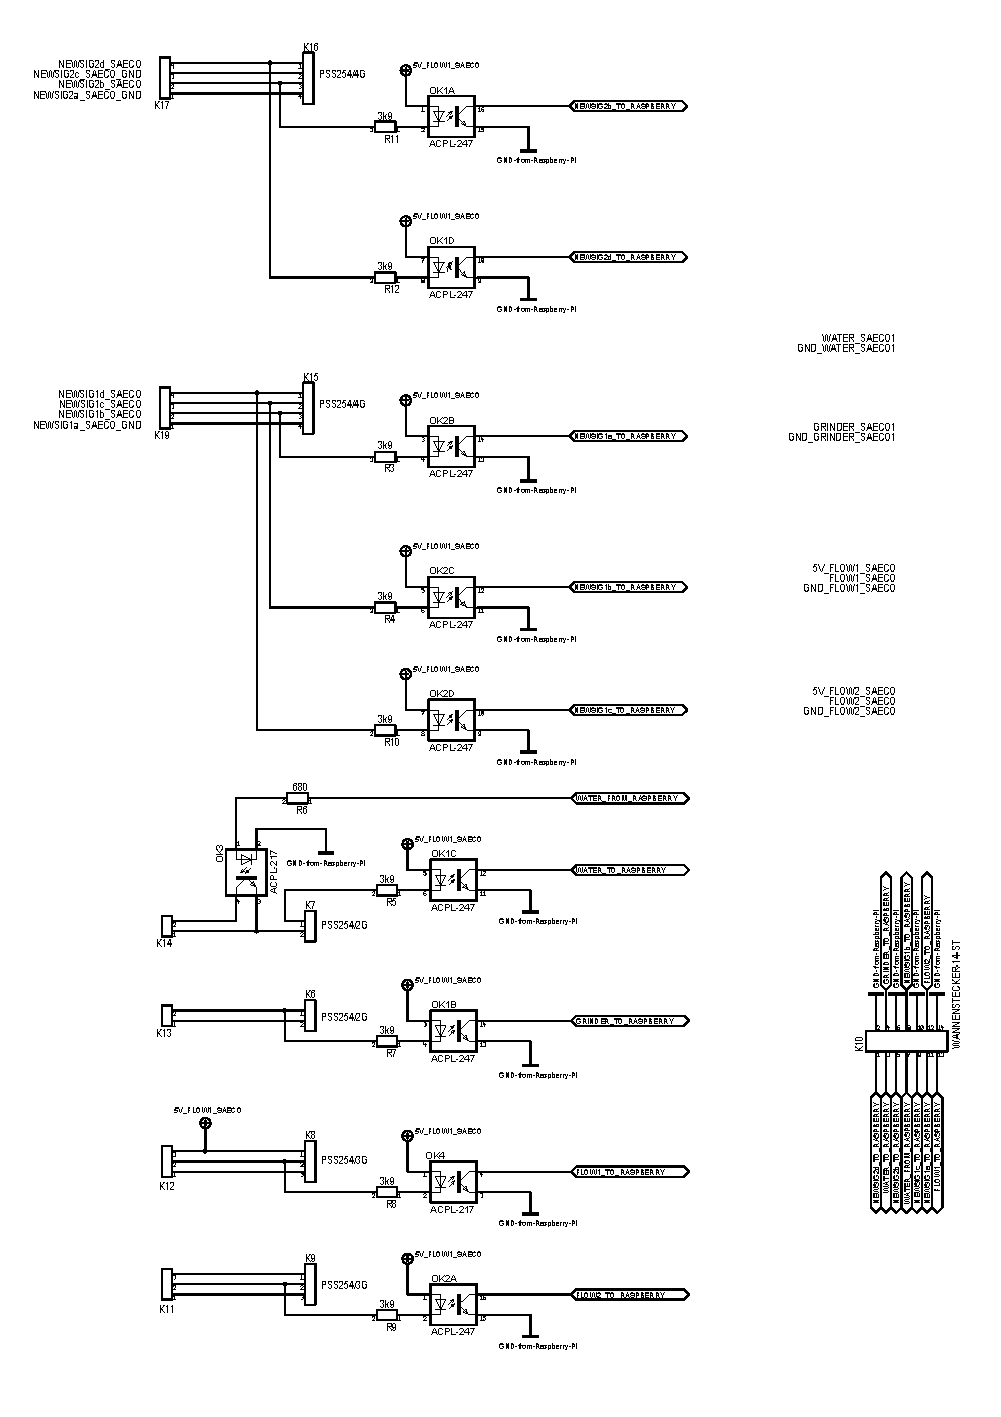
\includegraphics[width=15cm]{./images/pcbSchematic.pdf}
   \captionsetup{justification=centering}
   \caption{Schematic of the new PCB}
   \label{fig:newPCB}
  \end{figure}
  
\end{document}
